\documentclass[a4paper,12pt]{article}
\usepackage{tabularx} % extra features for tabular environment
\usepackage{amsmath}  % improve math presentation
\usepackage{float}
\usepackage{pdfpages}
\usepackage{cite}
\usepackage{multicol}
\usepackage{graphicx} % takes care of graphic including machinery
\graphicspath{ {./figures/} }
%\usepackage[margin=1in,letterpaper]{geometry} % decreases margins

\usepackage[final]{hyperref} % adds hyperlinks inside the generated pdf file
\hypersetup{
    colorlinks=true,       % false: boxed links; true: colored links
    linkcolor=blue,        % color of internal links
    citecolor=blue,        % color of links to bibliography
    filecolor=magenta,     % color of file links
    urlcolor =blue         
}
\usepackage[margin = 1in,headsep=0.5cm,headheight=2cm,letterpaper]{geometry} 
\usepackage{subcaption}

\usepackage{fancyhdr}

\usepackage{listings}
\usepackage{color}

\definecolor{dkgreen}{rgb}{0,0.6,0}
\definecolor{gray}{rgb}{0.5,0.5,0.5}
\definecolor{mauve}{rgb}{0.58,0,0.82}

\lstset{frame=tb,
  language=Python,
  aboveskip=3mm,
  belowskip=3mm,
  showstringspaces=false,
  columns=flexible,
  basicstyle={\small\ttfamily},
  numbers=none,
  numberstyle=\tiny\color{gray},
  keywordstyle=\color{blue},
  commentstyle=\color{dkgreen},
  stringstyle=\color{mauve},
  breaklines=true,
  breakatwhitespace=true,
  tabsize=3
}




\pagestyle{fancy}
\lhead{Intern: Ahmet Akman 2442366  \\ Supervisor: Dr. Johannes Zierenberg}
%\rhead{Date: \today \\ Duration: 19.07.22-21.08.22} 
%\cfoot{center of the footer!}
\renewcommand{\headrulewidth}{0.1pt}

\title{

\includegraphics[width=17cm]{odtu.png} \\

\includegraphics[width=4cm]{eee.png} \\
\vspace*{0.5in}
\textbf{EE400 Summer Practice Report}
\vspace*{0.25in}
}

\author{Intern: Ahmet Akman 2442366\\
Supervisor: Dr. Johannes Zierenberg\\
Supervisor Contact: \href{mailto: johannes.zierenberg@ds.mpg.de}{ johannes.zierenberg@ds.mpg.de. }-\href{tel:+495515176475}{+495515176475}\\
Assigned Faculty Member: Prof.Dr. Engin Tuncer\\
Institution Name: Max Planck Institute for Dynamics and Self-Organization\\
Start date:03.07.2023 || End date: 22.09.2023\\
        \vspace*{0.25in} \\
        Electrical and Electronics Engineering Department\\
        \textbf{Middle East Technical University}\\
        Ankara, Turkey
       } \date{\today}


\begin{document}

\bibliographystyle{plain}

%\thispagestyle{empty}
%\includepdf[pages=-]{coverpage_signed.pdf}


\maketitle

\newpage
\tableofcontents
\newpage
%\begin{abstract}
%abstract
%\end{abstract}
\section{Introduction}
\section{About Institution}
\subsection{Institution Name}
Max Planck Institute for Dynamics and Self-Organization.
\subsection{Institution Location}
Max Planck Institute for Dynamics and Self-Organization
Am Faßberg 17
37077 Göttingen
Germany
\subsection{General Description}
The Max Planck Institute for Dynamics and Self-Organization, located in Göttingen, Germany, is a prominent research institution primarily focused on the investigation of complex non-equilibrium systems, particularly within the fields of physics and biology. Its historical roots trace back to 1911 when Ludwig Prandtl initiated the establishment of a Kaiser Wilhelm Institute dedicated to the study of aerodynamics and hydrodynamics. This initial effort led to the formation of the Aeronautische Versuchsanstalt in 1915, which later evolved into the Kaiser Wilhelm Institute for Flow Research in 1924. In 1948, it became a part of the Max Planck Society. In 2003, it underwent a name change and became the Max Planck Institute for Dynamics and Self-Organization. Presently, it stands as one of the 80 institutes under the auspices of the Max Planck Society, contributing significantly to the understanding of intricate dynamic systems.

\subsection{Organization Structure}
The organization structure of the institute is given in Figure \ref{organization}. I was part of the group led by Prof.Dr. Viola Priesemann which is indicated as italic on \ref{organization}.

\begin{figure}[htb!] \centering{
    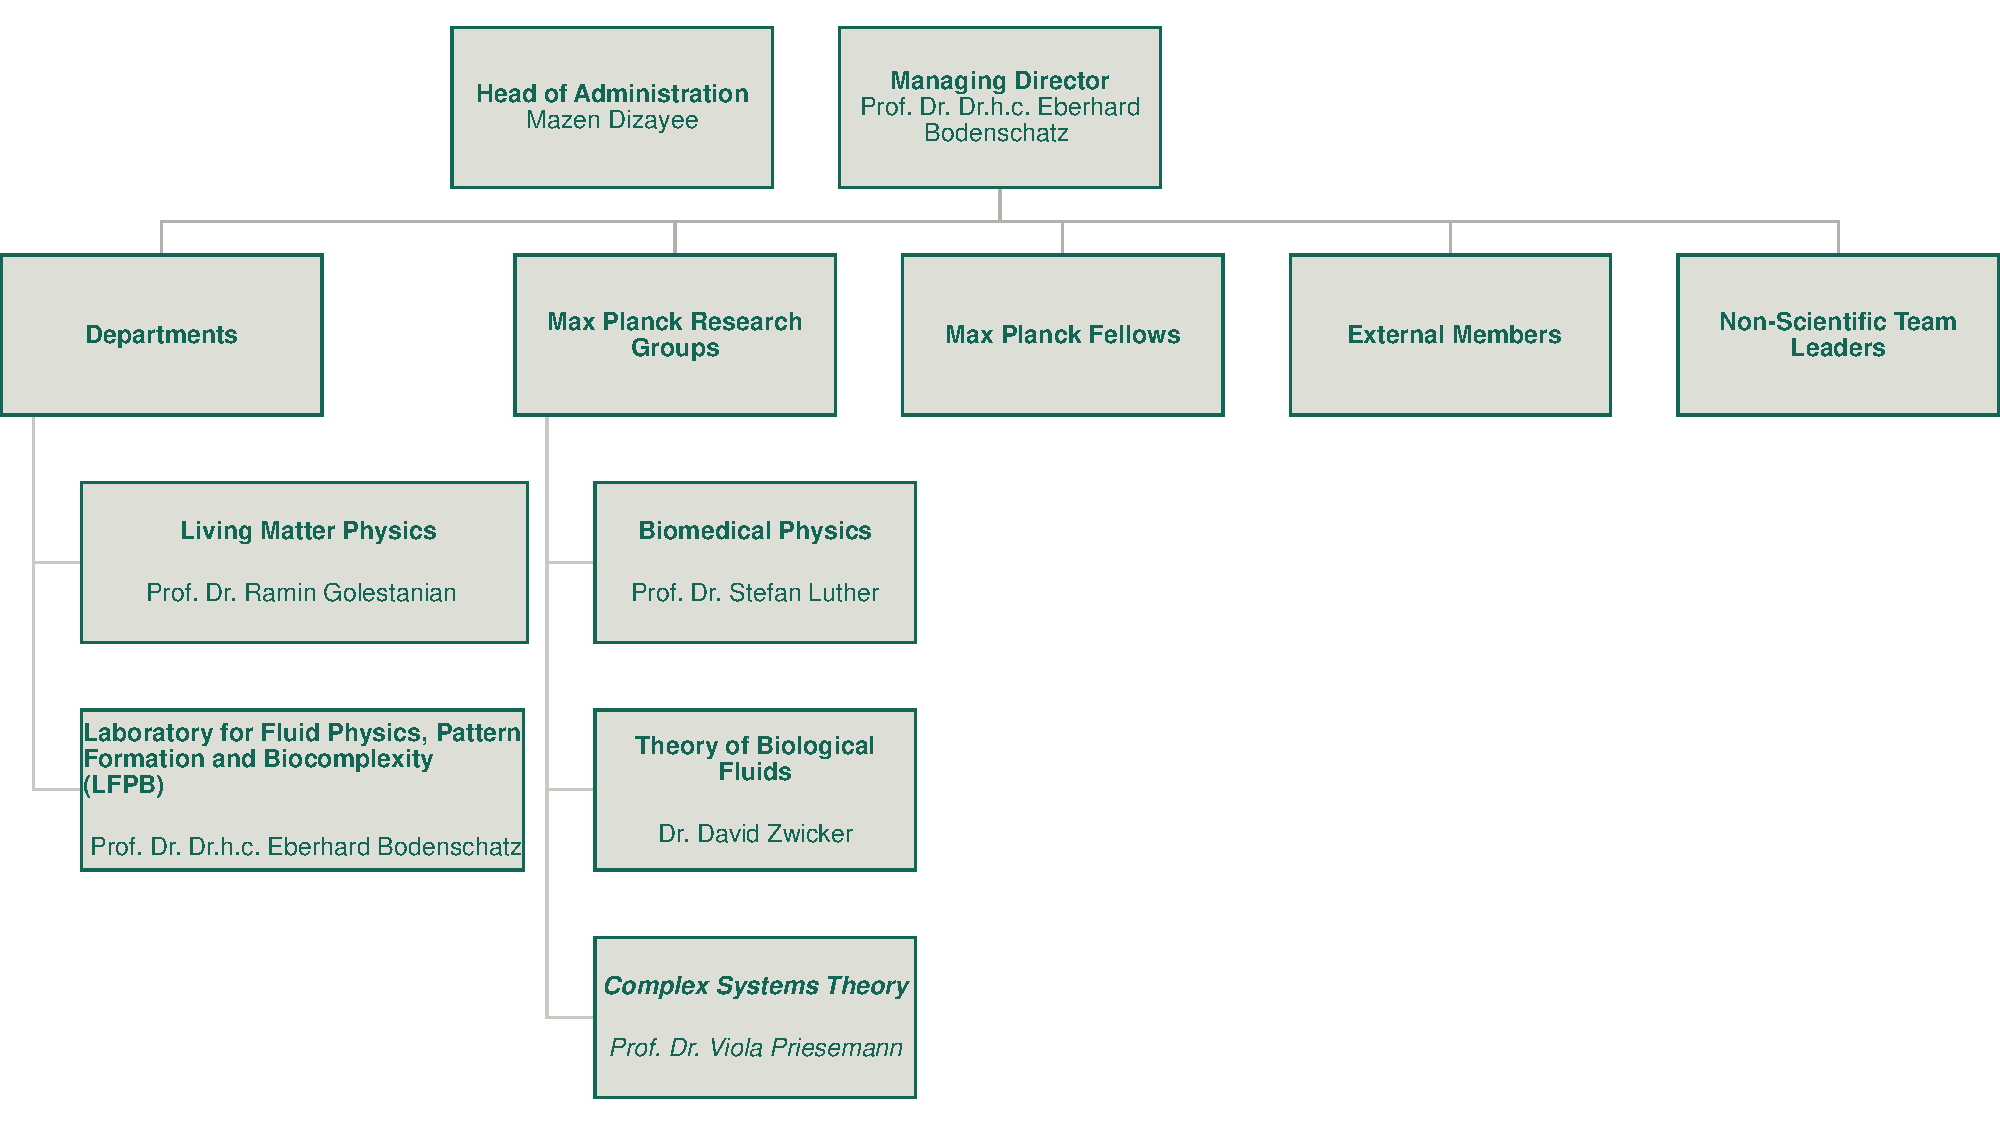
\includegraphics[width=\linewidth]{OrgChartMPIDS.pdf}}
    \caption{Basic organizational structure of MPI-DS.}
    \label{organization}
\end{figure}

\section{Project Background and Motivation}
The research project for the internship is constructed upon the following set of previous research. In the field of neuroscience \cite{CHAOS}, initiated the idea of inhibition is a necessary part of a neuronal network for stability of the network. Then, the impactful paper \cite{brunel} explained the dynamics of a sparsely connected random network with fixed parameters. Also, the role of inhibition was similar to the \cite{CHAOS}. The phases of the network through these dynamics are also stated. These states can be summarized as follows also givein in Figure \ref{brunel_fig}. Synchronous regular (SR) is the state where the whole network is blinking in a synchronized way. So, the neurons are synchronized with each other, exciting each other together, and regular activity is observed. Synchronous irregular (SI) is the state where the individual neurons show irregular activity, but the global activity is still regular. Therefore, the rate of the random network is still blinking in some sense. SI-fast and SI-slow characterize this as two different dynamical states. The asynchronous irregular state is the desired stable state where both the individual (per-neuron) and global activity show irregularity, that is, to small average overall activity not-blinking global network. \cite{brunel} has been considered as a guiding baseline in the field, and many other network descriptions built upon this idea, including inhibition as a factor for stability. It is important to note that the \cite{brunel} employs a fixed set of parameters on a completely randomly connected network.

\begin{figure}[htb!]
    \centering
    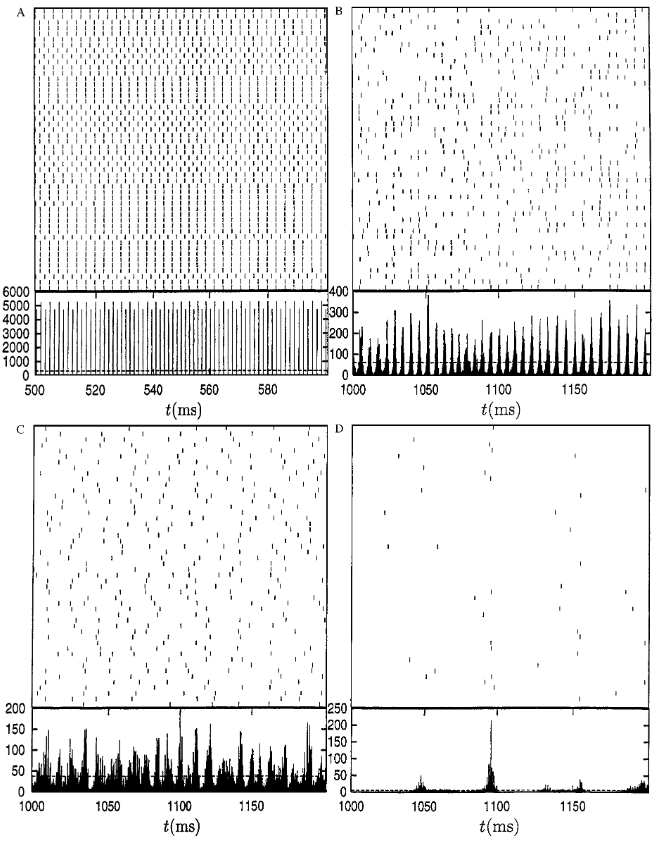
\includegraphics[width = 0.5\textwidth]{brunel.png}
    \caption{The states of the network. (A) Synchronous Irregular. (B) Synchronous Irregular-fast. (C) Asynchronous Irregular. (D) Synchronous Irregular-slow.}
    \label{brunel_fig}
\end{figure} 

\subsection{Hypothesis}

In neurobiology, one can classify the neurons as excitatory and inhibitory. A typical excitatory neuron is called a pyramidal neuron, whereas there are more than 20 mainstream types of inhibitory neurons. The idea is that the role of inhibition might be something other than just stabilizing the network. So, we hypothesize that only excitatory networks can be stable. To achieve the stability, the structural connectivity of the network should be reconsidered. \cite{2Dstructure} describes the 2D layered structure of the cortical networks in the brain. 

\section{Project Description}
The project is built upon the hypothesized idea frame. First, the tools for the project are determined. For simulation implementation, Python programming language and a brain simulator package called Brian2 \cite{brian2} are used. The simulations run on the HPC (High-performance computing cluster.), which is set to be used with the industry standard SGE (Sun Grid Engine). The project timeline aligns with the report format presented in this document. 

\subsection{2D Connectivity}
The 2D locality of the network is somewhat intuitive as the neurons in the cortical networks have a higher probability of connection to nearby neurons. In order to model this phenomenon, first, the $N$ number of neurons is randomly located in the $1 by 1$ area. Then, according to the "smallest distance" between each pair, the probability map is constructed by zero-mean Gaussian. Figure \ref{prob_map} gives an example probability map for $N = $. In this formulation, the outdegree $K$ of the neurons is fixed. That is to say, one neuron has a fixed number of outgoing connections. In other words, one axon has a fixed number of synapses. According to the probability map, the connection assignment process is conveyed as picking $K$ number of neuron $j$'s to connect neuron $i$ without replacement. A sample is given in Figure \ref{connectionmap}.

\begin{figure}[htb!]
    \centering
    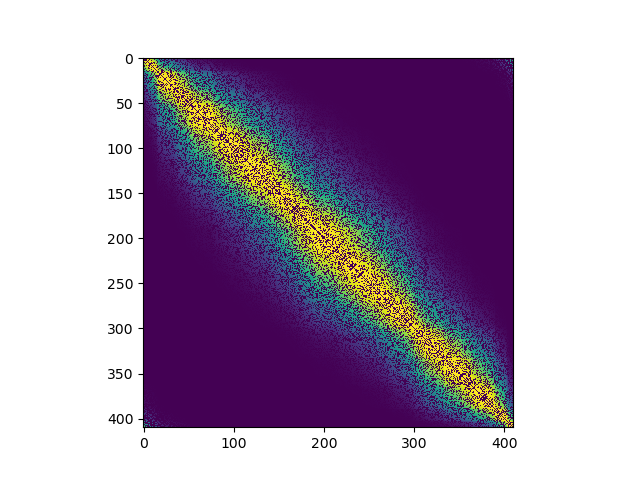
\includegraphics[width = 0.75\textwidth]{prob_map.png}
    \caption{Sample probability map for $N = 512$}
    \label{prob_map}
\end{figure} 

\begin{figure}[htb!]
    \centering
    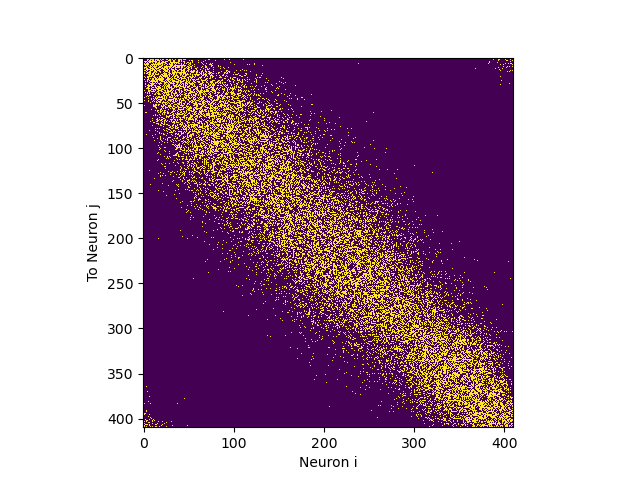
\includegraphics[width = 0.75\textwidth]{connections.png}
    \caption{Sample connection map for $N = 512$}
    \label{connectionmap}
\end{figure} 
Also, the connections for one neuron are illustrated in Figure \ref{neuron_network} as a part of the whole network for $N=10000$ and $K=100$, which is the standard network size through the rest of the study.

\begin{figure}[htb!] \centering{
    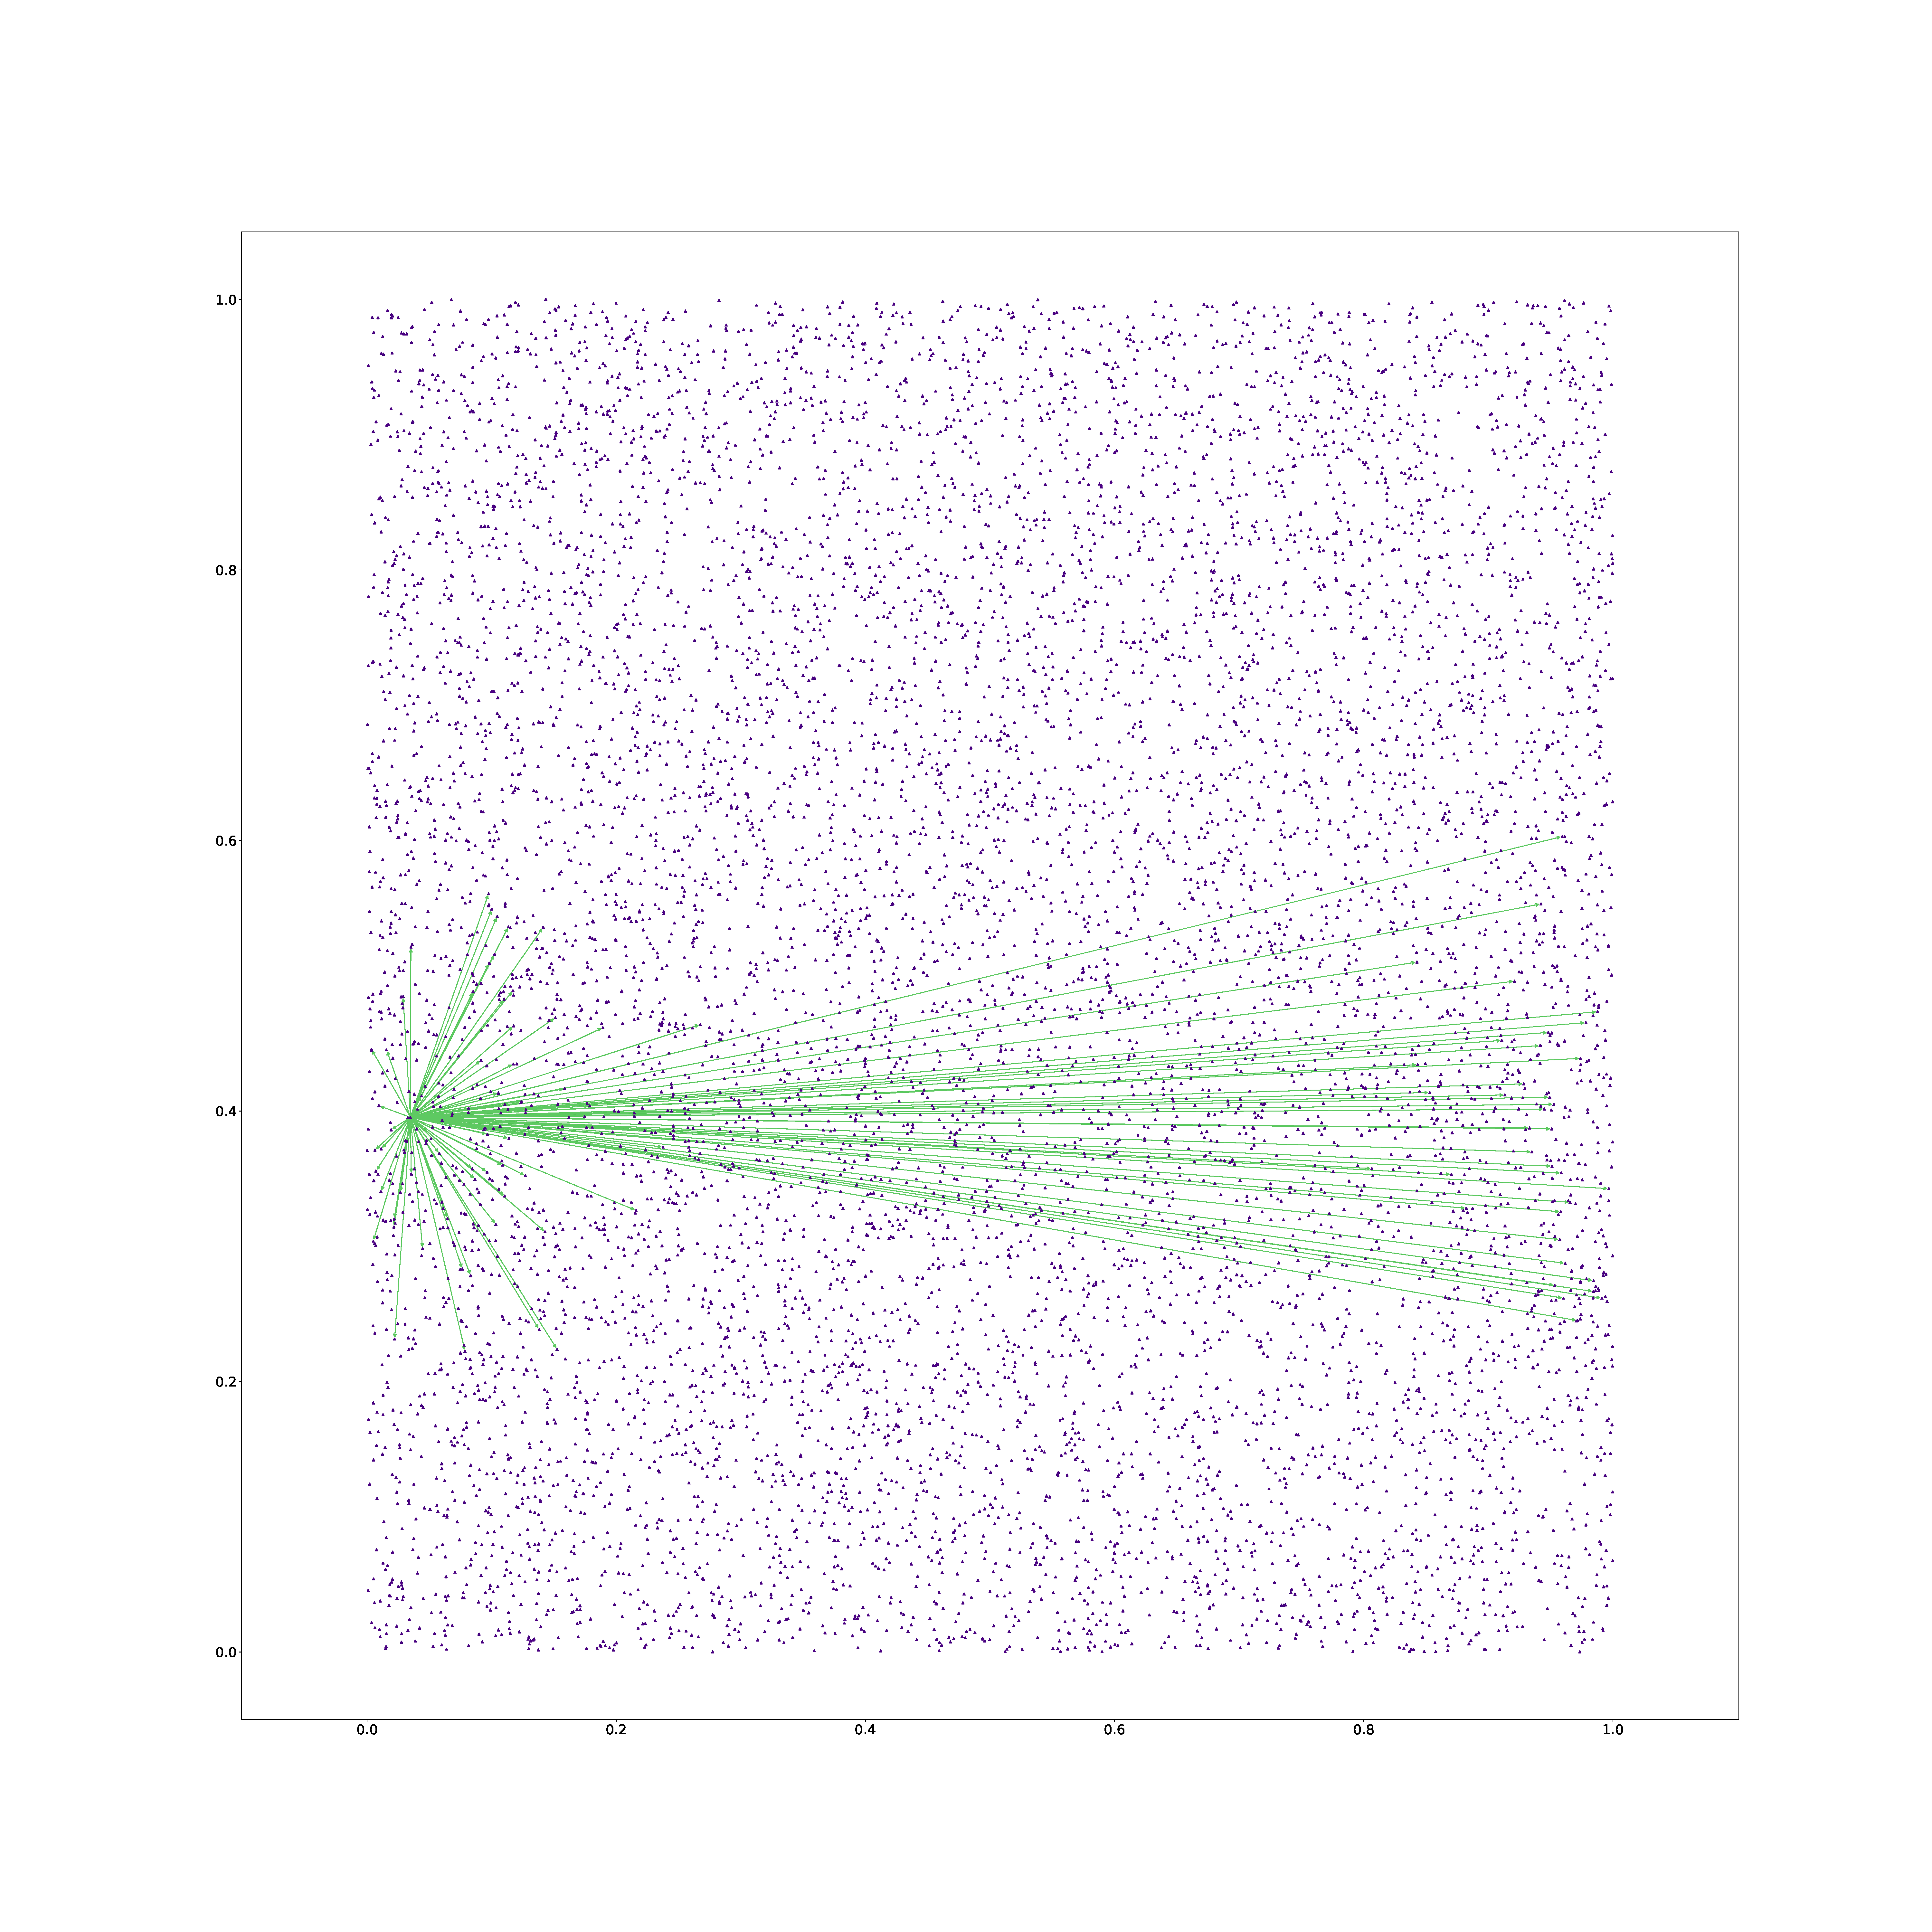
\includegraphics[width=\linewidth]{neuron_network.pdf}}
    \caption{Connections of a neuron on the bigger network size.}
    \label{neuron_network}
\end{figure}


There are two important points that should be stated. First, the "smallest distance" is being calculated as if the 2D plane has periodic boundary conditions, creating 3D torus structure. Second, as the outdegree is fixed the $\sigma$ value, which is the standard deviation of the Gaussian function has two limitations. One dependent on the system size, the other one is dependent on the outdegree. Since the periodic boundary conditions apply, larger $\sigma$ loses its effectiveness. On the other hand, as the $\sigma$ goes smaller and smaller it becomes impossible distinguish between two different values because of the fixed number of selections, so one can not go more local in that sense. To be able to illustrate this situation the Figure \ref{effectivesigma}. On x axis the $\sigma$ value for the probability map is ranged. On y axis the $effective \text{ } \sigma$ which is the average distance of the connected neurons, is given. This plot allowed us to choose a small and useful enough $\sigma$ value. 
\begin{figure}[htb!] \centering{
    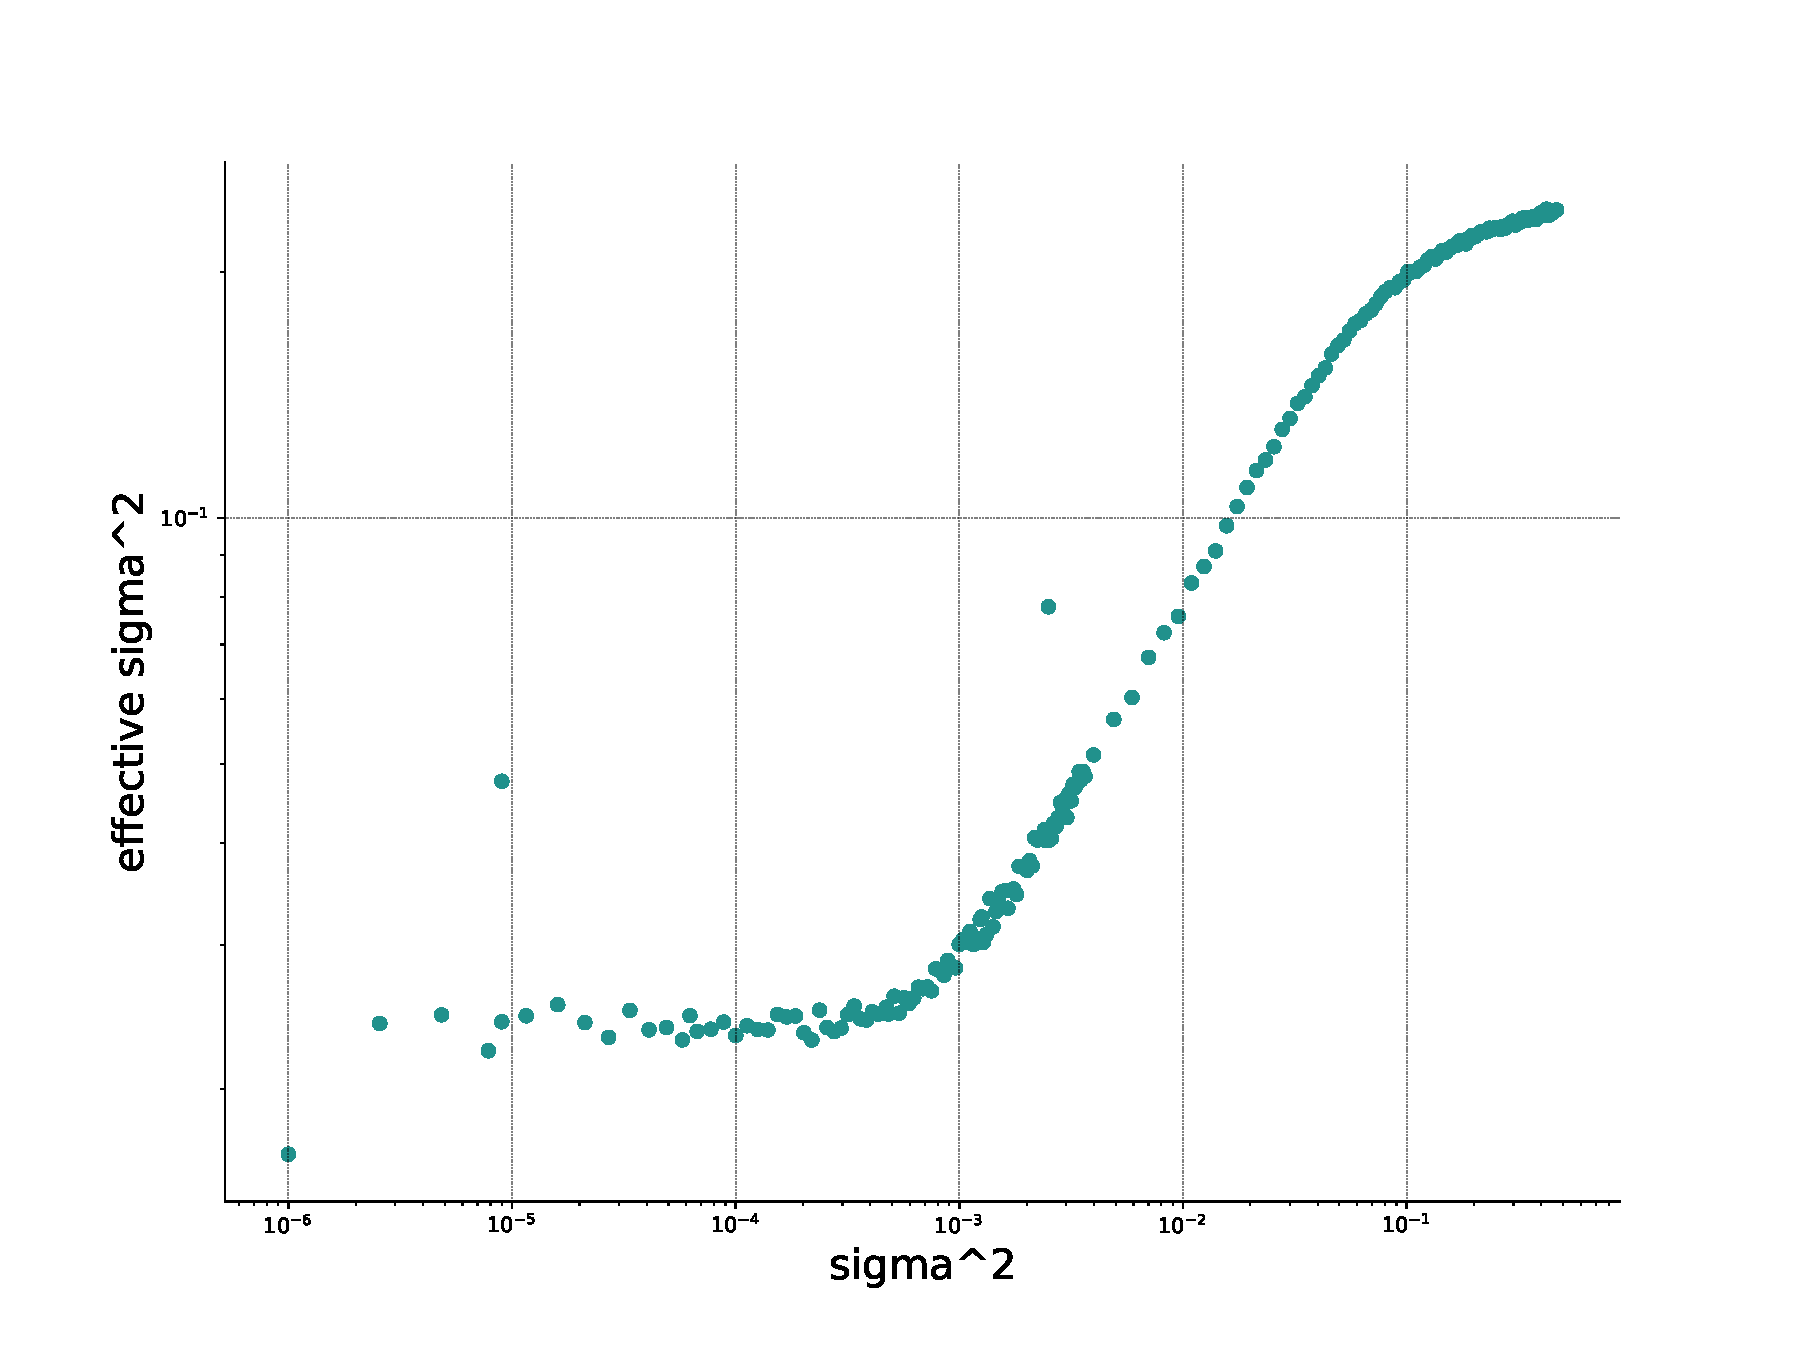
\includegraphics[width=\linewidth]{K_rec100_N_10000_K_rec100_N_10000.pdf}}
    \caption{effective $\sigma ^2$ vs $\sigma ^2$.}
    \label{effectivesigma}
\end{figure}



\subsection{Baseline}


First, the simulations that form a basis are conveyed before introducing regulative mechanisms. Let us build our model one by one. The differential equations that determine the behavior of a neuron are given in equation \ref{diff_eqn}

\begin{equation}
    \begin{split}
        \frac{dv}{dt} & = -\frac{(v - v_{leak_i})}{\tau_{mem_i}}+ noiseparam \times sqrt(\frac{2}{\tau_{mem_i}}) \times xi \\
        \frac{dI_{exc}}{dt} & = \frac{I_{exc}}{\tau_{exc_i}}
    \end{split}
    \label{diff_eqn}
\end{equation}
The main parameters are taken from \cite{brunel} for consistency. The parameters and the maximum noise value are given in Table \ref{parameterset}. This is the model for spiking neurons as the $v_{thres}$ exceeded the neuron spikes and the membrane voltage returns to the reset value. The $d_{\text{syn}}$ is the axonal delay parameter where the spikes take their time to reach the destination neuron. The $\tau_{\text{ref}}$ corresponds to the refractory period in which the neuron can not spike for that amount of time after spiking. The reversal parameter is implemented in order to scale the code easily in case of introduction inhibition. So, if a neuron gets too much inhibition in a time interval, the reversal parameter can not exceeded. That is biologically realistic since, in such a situation, the synaptic interface gets saturated.

\begin{table}[h]
    \centering
    \begin{tabular}{|c|c|c|}
    \hline
    Parameter & Value & Maximum Noise \\
    \hline
    $\tau_m$ & 20.0 ms & 1.0 \\
    $\tau_{\text{syn\_exc}}$ & 5.0 ms & 0.2 \\
    $v_{\text{leak}}$ & 0 mV & 0 \\
    $v_{\text{thres}}$ & 20 mV & 0.5 \\
    $v_{\text{reset}}$ & 10 mV & 0.5 \\
    $\tau_{\text{ref}}$ & 2 ms & -- \\
    $d_{\text{syn}}$ & 1.5 ms & -- \\
    $v_{\text{rev}}$ & -10.0 mV & reversal \\
    \hline
    \end{tabular}
    \caption{Parameter Values}
    \label{parameterset}
\end{table}
It should be noted that different from \cite{brunel}, temporal and parameter noise is involved in our model in order to make it stochastic, thus realistic. Also, to make sure that introducing $\% 5$ noise does not make the system deviate from where it should be, the simulations are also run in no-noise settings, and it is verified that the variability does not make the system go crazy.

As we have compiled our basic neuronal model, the coupling parameter $J$ is swept through different values in order to find the threshold where the neuronal activity jumps. The activity is measured as a rate per second per neuron from a few milliseconds of the simulation. Therefore, the resultant rate gives necessary information about sustaining activity. In this baseline, the external drive can be summarised as follows. For 5 seconds, each neuron gets a very high external Poisson rate of excitation. So, the network gets charged up. Then, the external drive was suspended, and the simulation continued for 15 seconds. As a result, the $J(mV)$ vs activity plot presented in Figure \ref{jvsactivity} is obtained. Also, when we zoom in on the time development of the four closest points to the jump point, as presented in \ref{ratevstime}, one can see that even though each network settles for a small amount of time to an intermediate non-full-bursting state, two of them dies out afterward. 
\begin{figure}[htb!] \centering{
    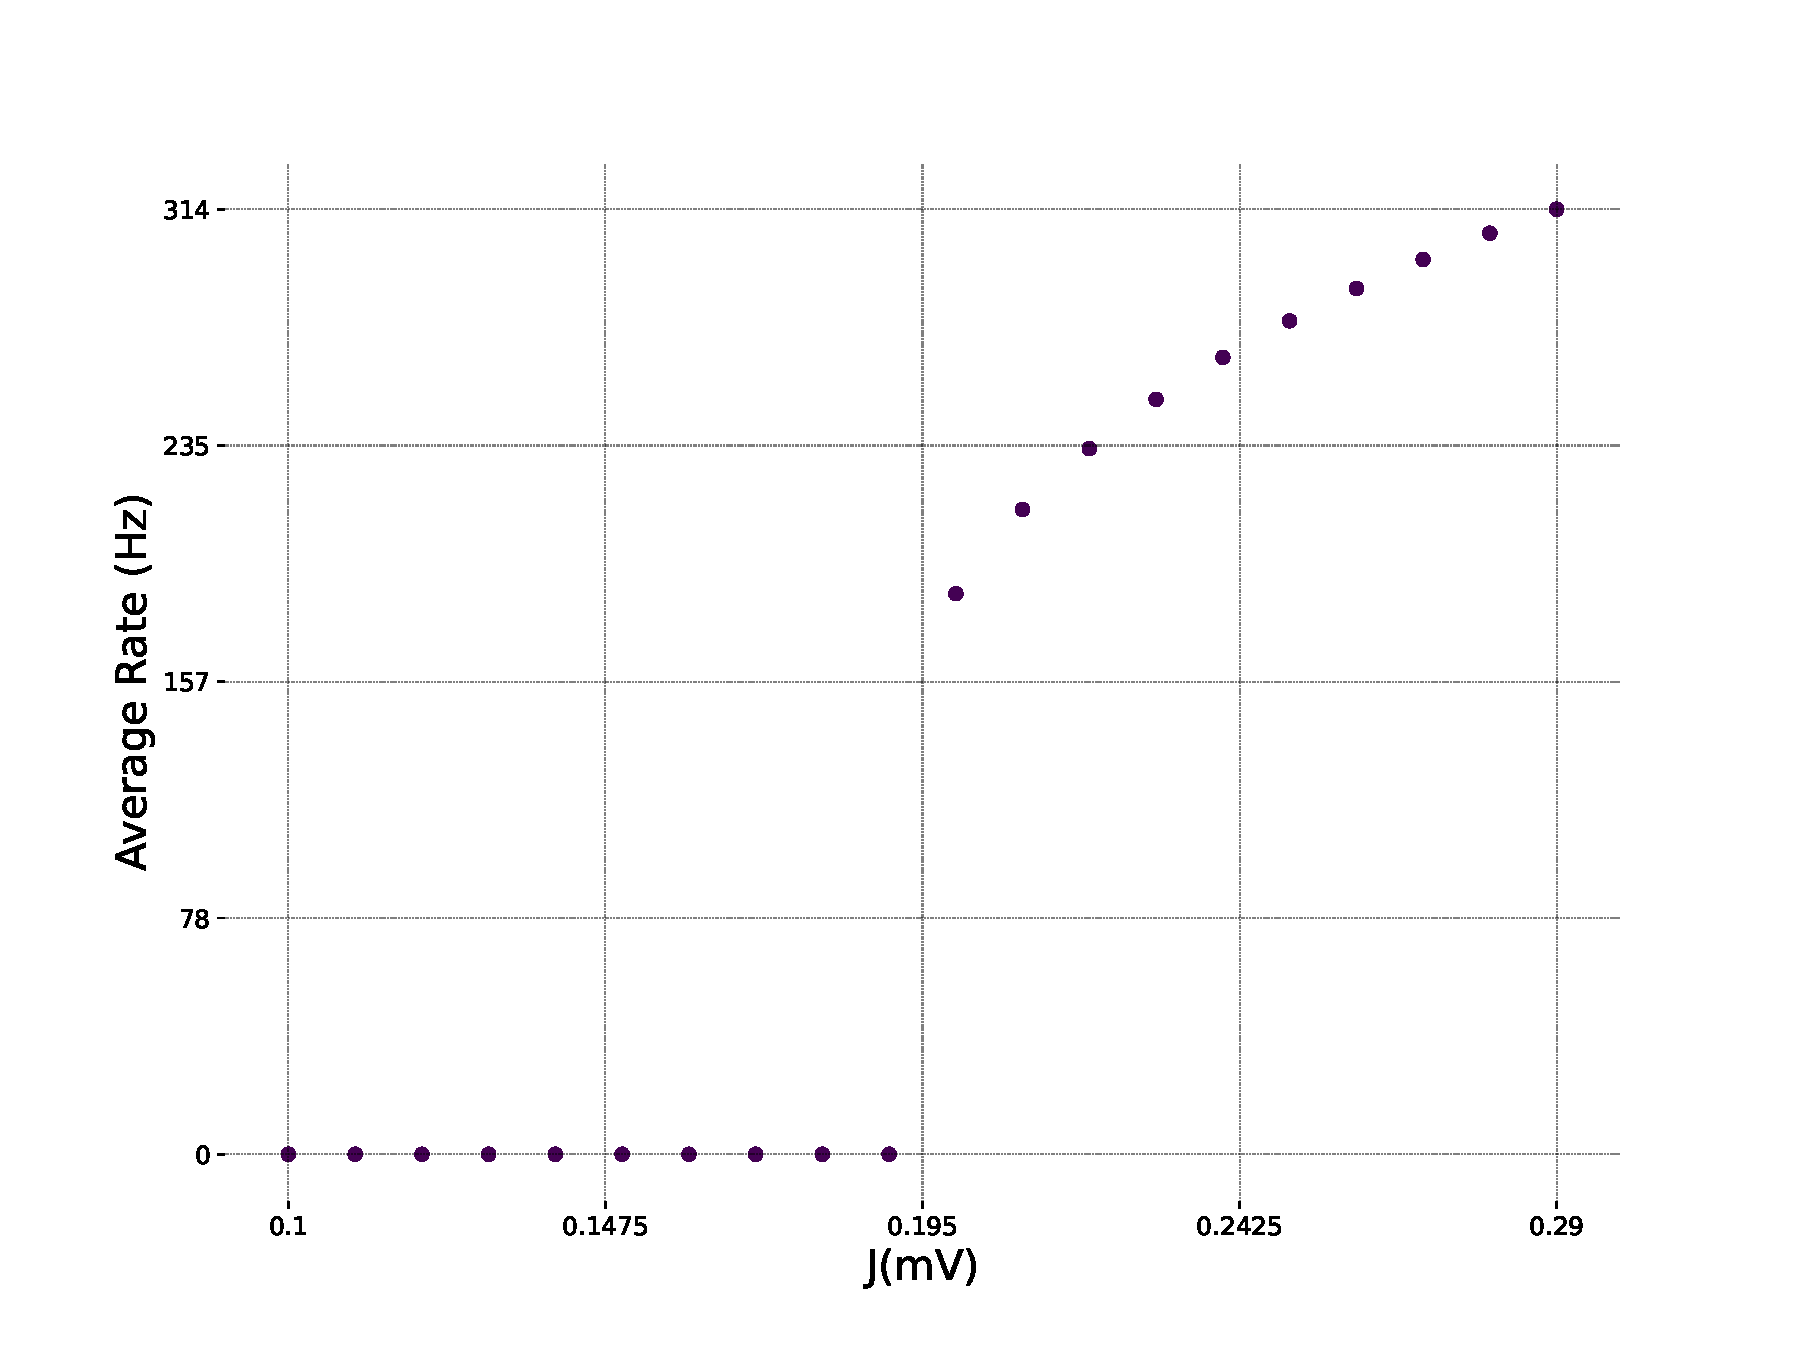
\includegraphics[width=\linewidth]{J_vs_activity.pdf}}
    \caption{Rate (Hz) vs J(mV) for baseline.}
    \label{jvsactivity}
\end{figure}

\begin{figure}[htb!] \centering{
    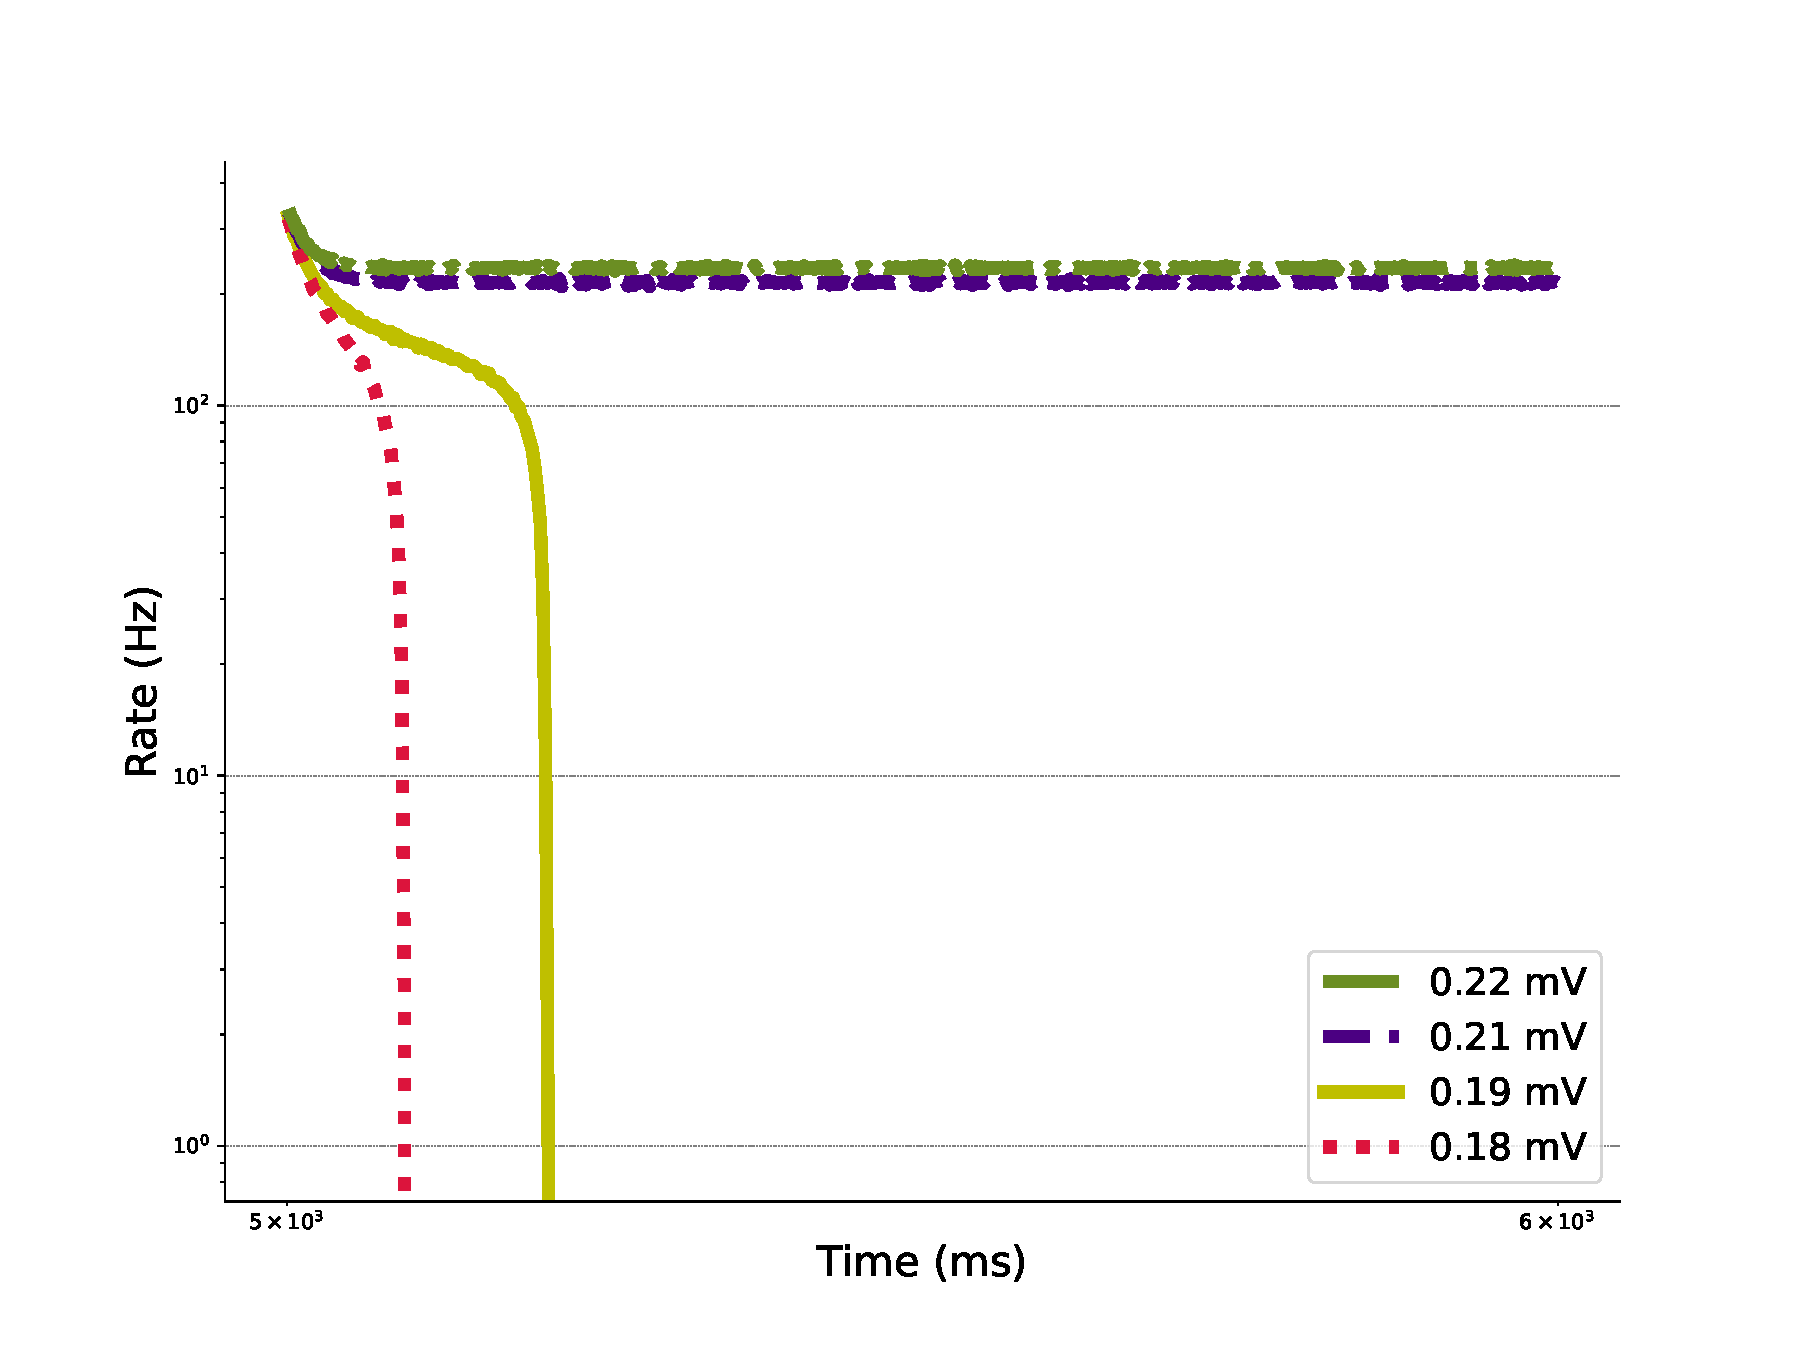
\includegraphics[width=\linewidth]{time_vs_activity.pdf}}
    \caption{Rate (Hz) vs time (ms) for baseline samples in logscale.}
    \label{ratevstime}
\end{figure}

The project is steered towards employing regulatory mechanisms for coupling parameter $J$ by forming a baseline.


\subsection{Homeostastatic Regulation}
Homeostatic regulation is a basic mechanism that is rooted in neurobiology. The idea is to use a local mechanism for each neuron to adjust its synaptic couplings (weights) according to the target firing rate. 

First, a basic homeostatic regulation mechanism adjusts a membrane quantity $\alpha$ multiplied by the $J$ for every synaptic connection. However, this uniform parameter is not realistic and valuable for two reasons. First, it is known that some synapses have more influence on the membrane potential than others. Second, mathematically, it is not much different than the fast way of adjusting each $J$ parameter per neuron by hand. So, the following formulation for each synapse is followed for homeostatic regulation (adaptation). 

The synapse model is constructed as given in \ref{eqnhome}. So then, each $J_i$ gets regulated. As can be observed from the baseline step, the system needs some level of energy in order to start spiking at a considerable rate. Therefore, different external poison excitation rates are applied. The target rate is set to 10 Hz. 
\begin{equation}
    \begin{split}
        \frac{dJ}{dt} &= A_c \times \frac{J-A_c}{\tau_{hp}} \\
        &\text{when a spike arrives at the postsynaptic neuron} \\
        J &= \frac{(J-A_c)}{\tau_{hp}} \\
        &\text{when a spike arrives at the presynaptic neuron}\\
        I_{exc} &= I_{exc} + J \text{  mV} \\
    \end{split}
    \label{eqnhome}
\end{equation}

Now that we have formulated our homeostatic steps, let's look at the results obtained. First, notice that there are more than one set of points. The reason is to be able to keep the 2D locality as a comparison element. The two simulations are run simultaneously. The simulations are named by the aviation alphabet to keep track of them more manageable when we have more than a few setups. The "Charlie" simulations (indicated by the color yellow) have a 2D Gaussian local structure. The "Sierra" simulations (indicated by the color indigo.) are the ones with randomly assigned networks. However, the fundamental setup measures, such as a number of external inputs and outdegree, were kept identical. Figure \ref{charlie} shows the plot that illustrates external input versus average rate. It can be said that the system is primarily input-driven. However, the target rate is approximated around the point $\nu_{ext} = 76$, creating a small plato. 
\begin{figure}[htb!] 
    \centering
    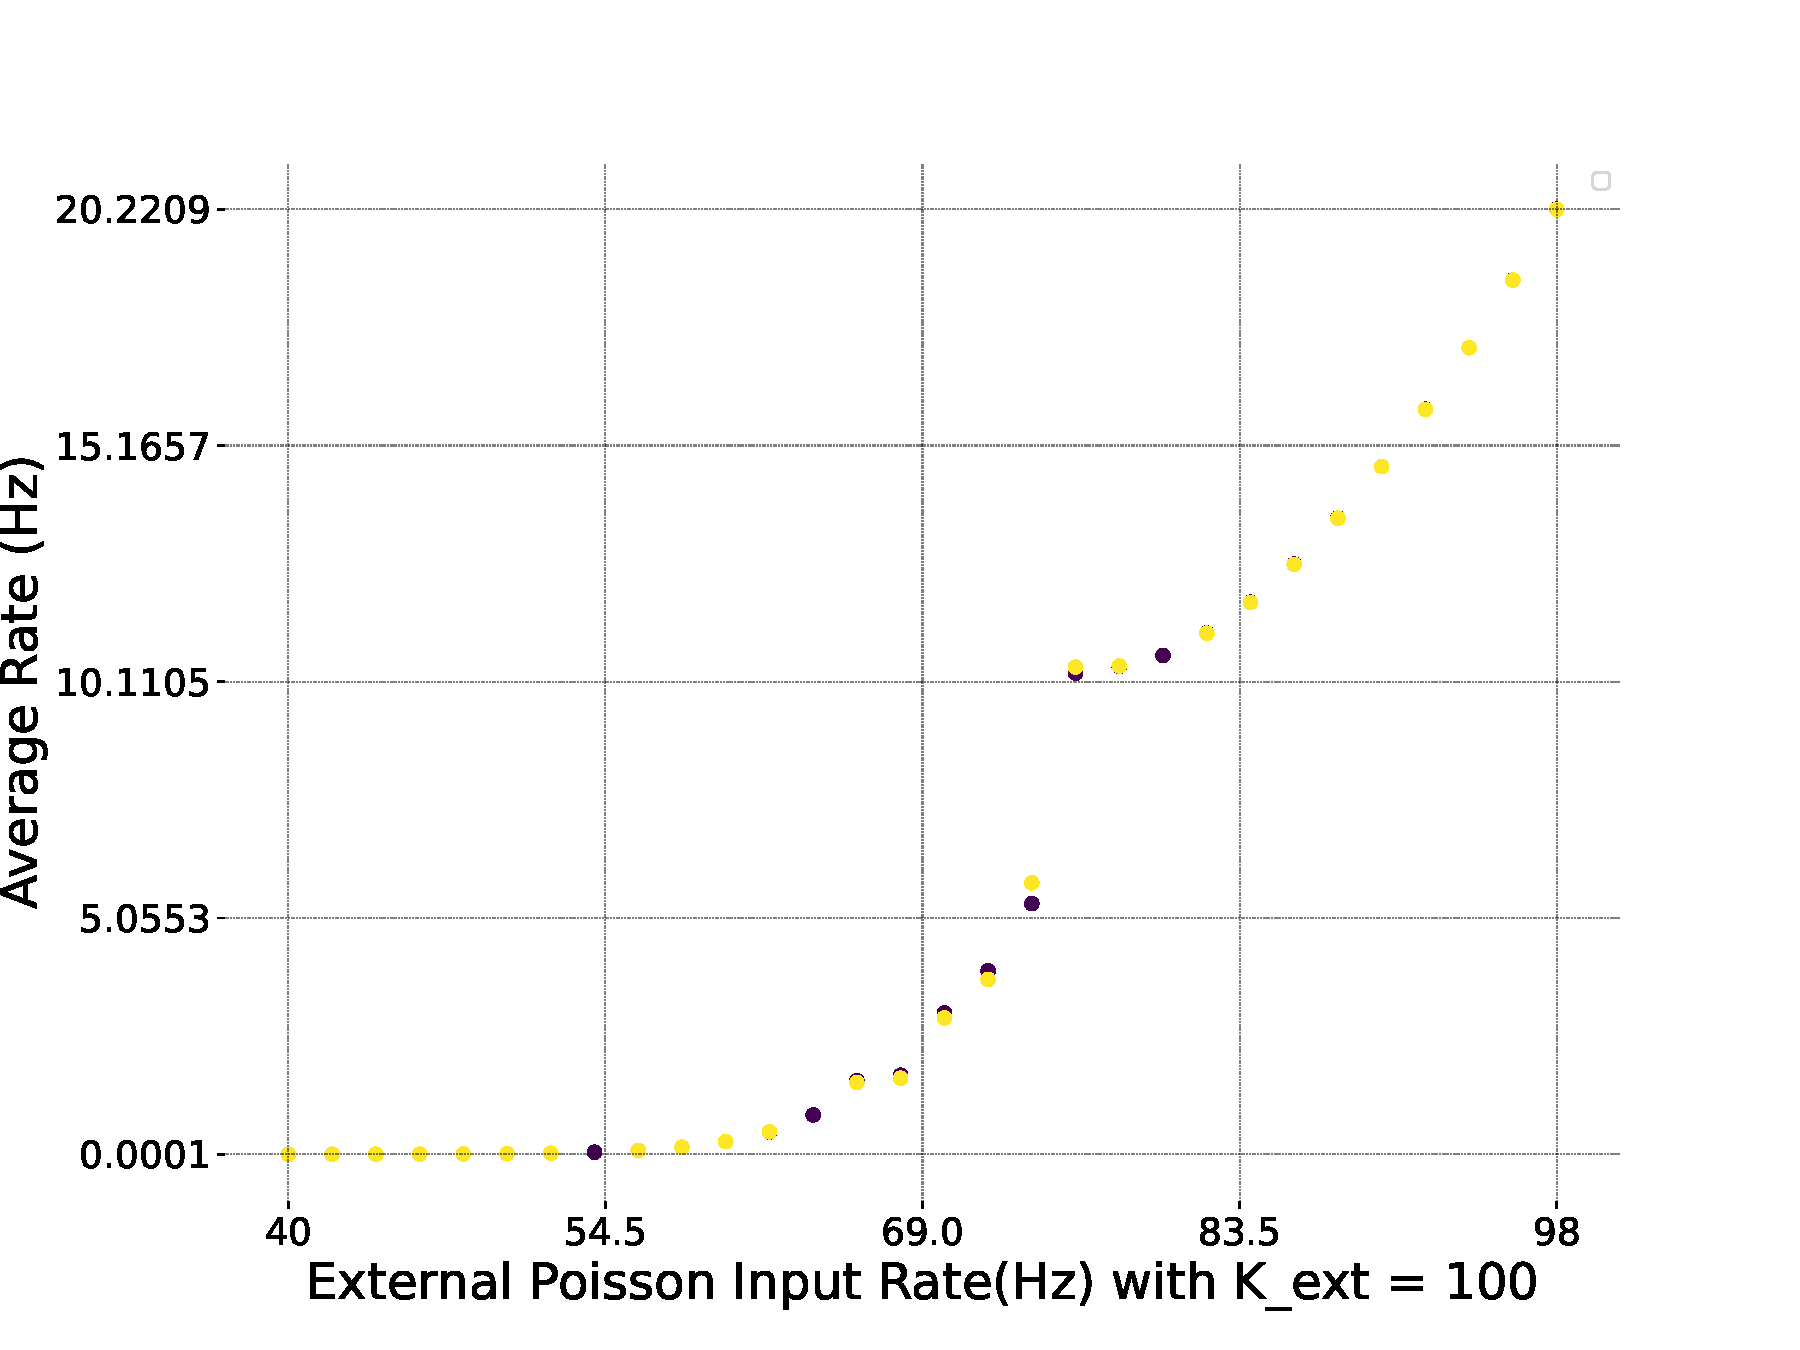
\includegraphics[width=\linewidth]{nuext_vs_activity_charlie.pdf}
    \caption{$\nu_{ext}$ vs Rate (Hz).}
    \label{charlie}
\end{figure}
In figure \ref{charlie76ratevstime}, the rate versus time plot for $nu_{ext} = 76$ is shown. It can be seen that even though some bursts occur after 100e6 milliseconds, the system tries to settle for 10 Hz.
\begin{figure}[htb!] 
    \centering
    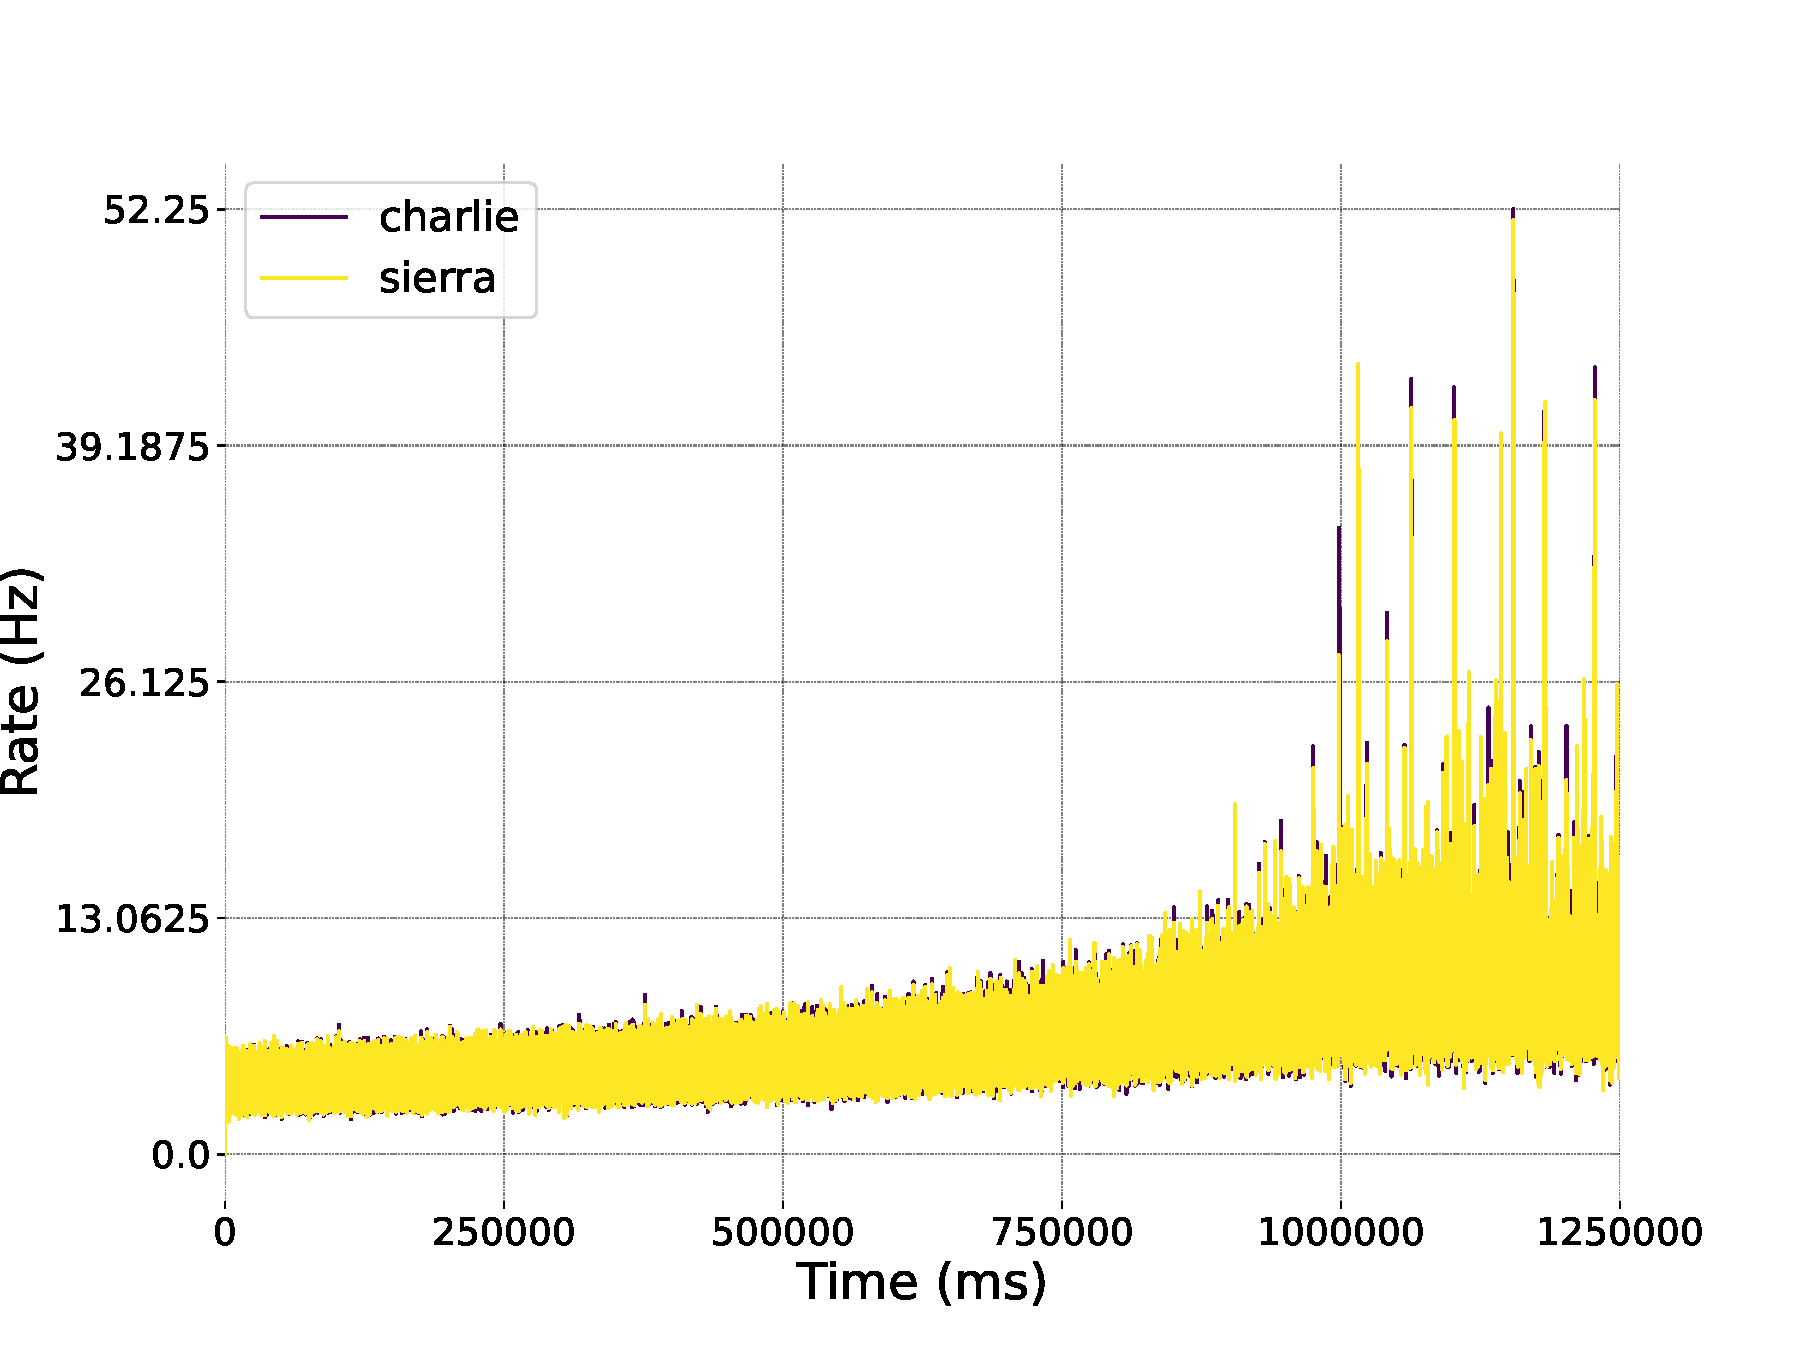
\includegraphics[width=\linewidth]{nu_ext_76rate_over_time_homeostasis.pdf}
    \caption{Rate (Hz) vs Time (ms)}
    \label{charlie76ratevstime}
\end{figure}
In order to observe the evolution of $J_i$, it is given in Figure \ref{charlie76alphavstime}. As one can see from the plot, the averaged J value converges to a fixed value. 
\begin{figure}[htb!] 
    \centering
    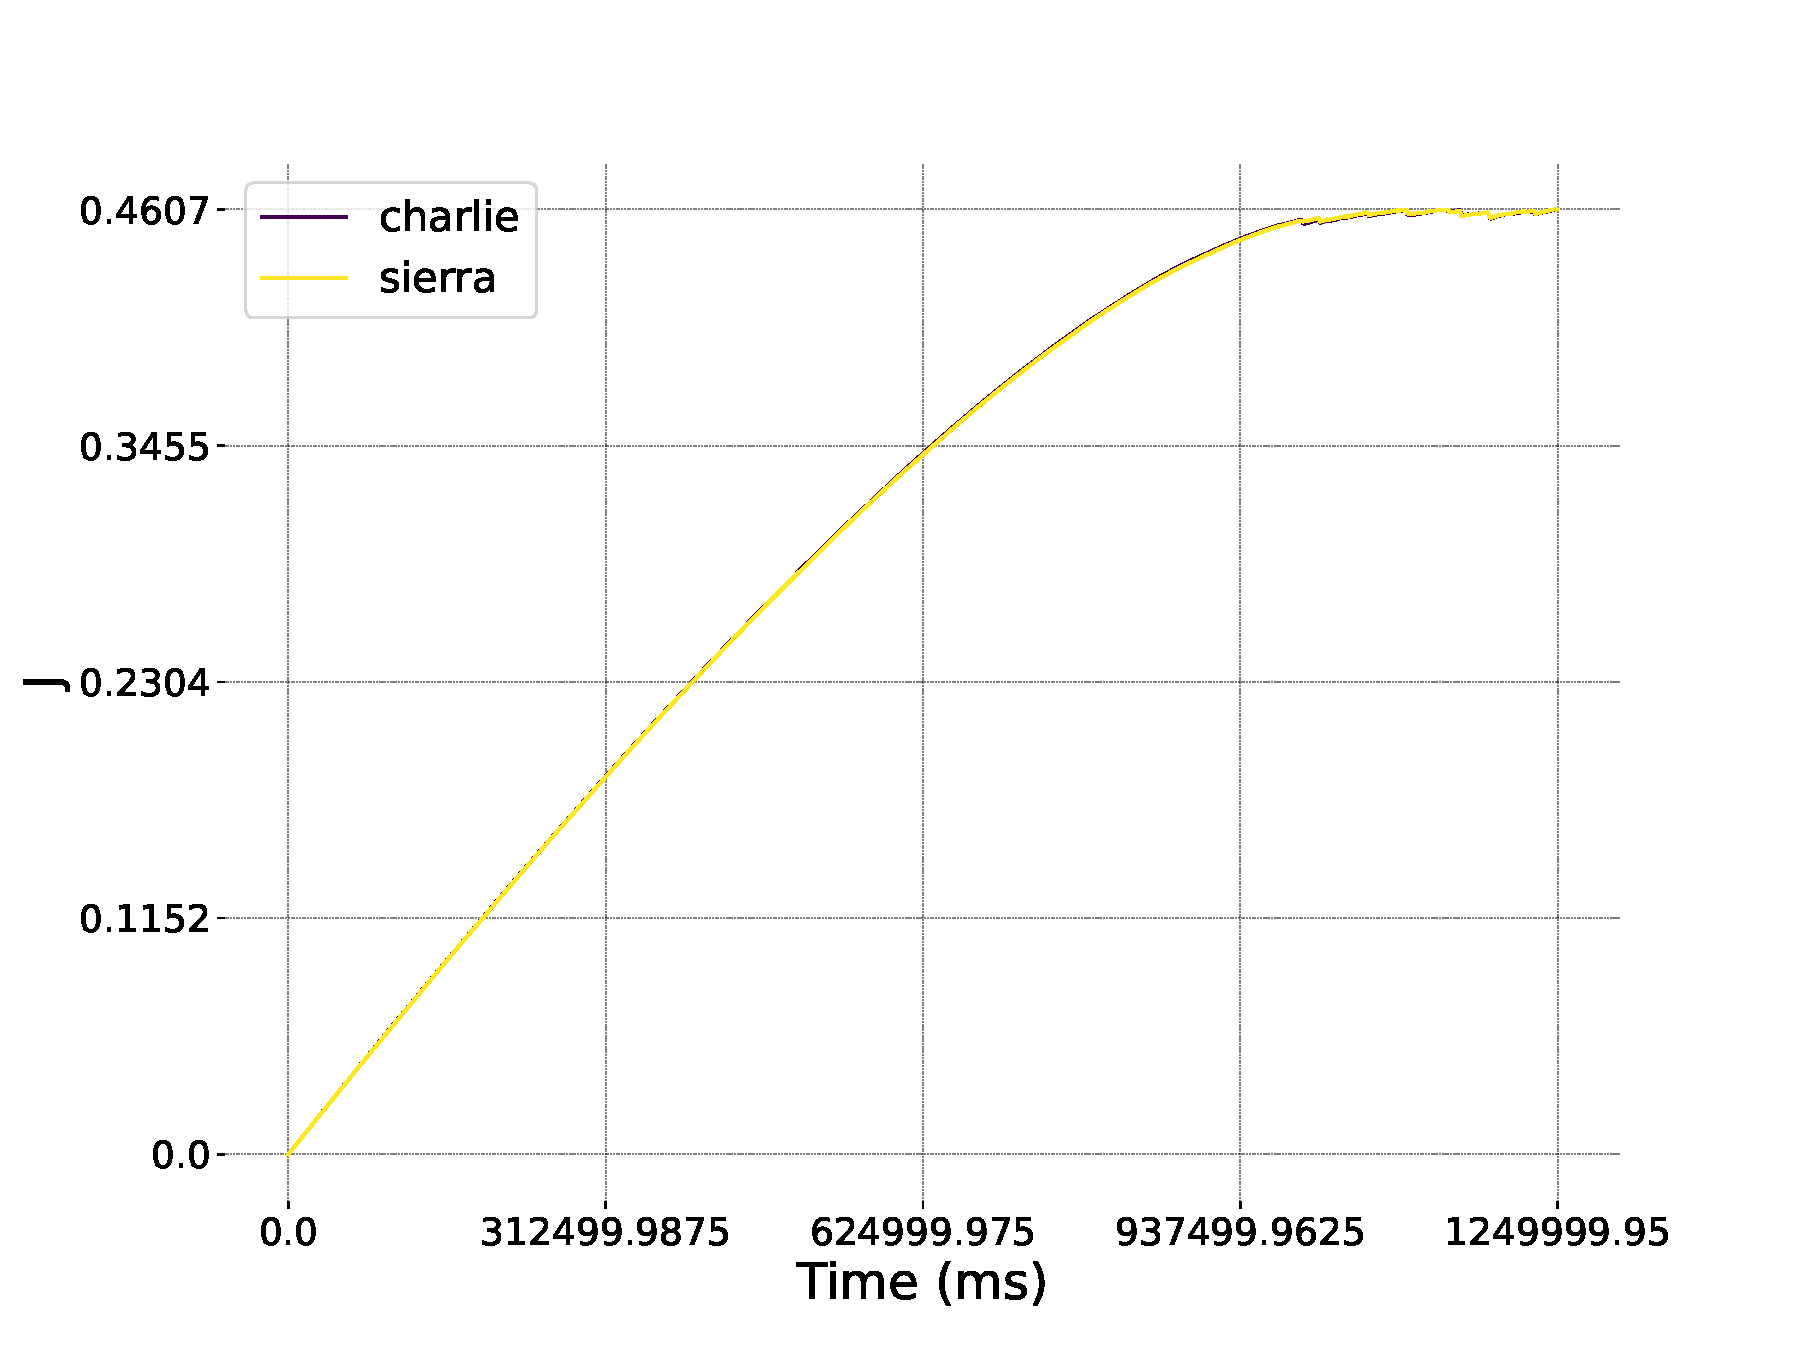
\includegraphics[width=\linewidth]{nu_ext_76alpha_over_time_homeostasis.pdf}
    \caption{ J (mV) vs Time (ms)}
    \label{charlie76alphavstime}
\end{figure}
Also, the Figure given in \ref{charlie76histogram} illustrates the final distribution of $J_i$'s. This plot tells us that a considerable amount of connnections die out, and there is a Gaussian-like distribution of coupling strengths.
\begin{figure}[htb!] 
    \centering
    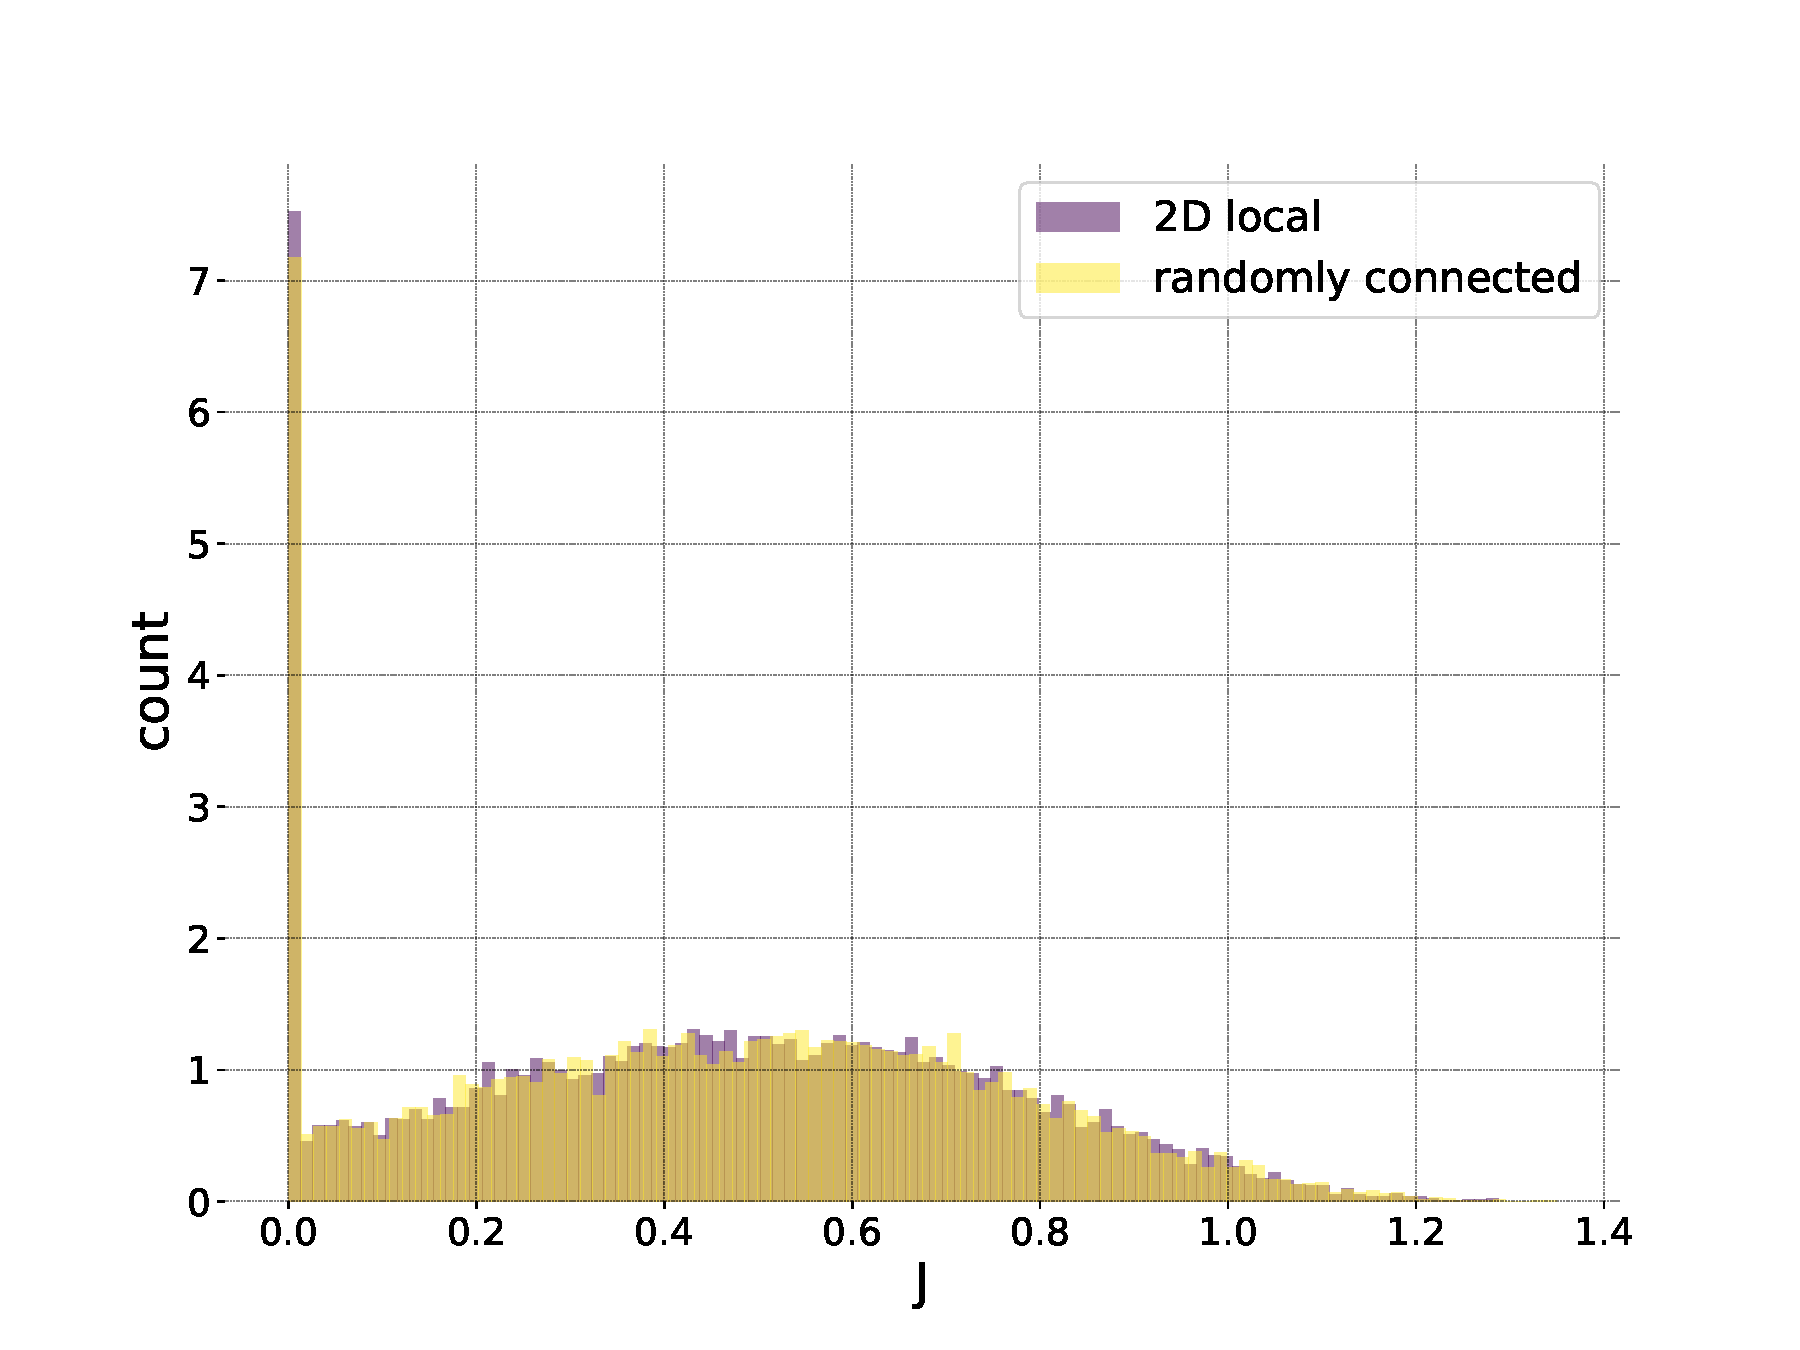
\includegraphics[width=\linewidth]{nu_ext_76j_dist.pdf}
    \caption{Distribution of J's}
    \label{charlie76histogram}
\end{figure}
To be able to understand the steadiness of the rate signal, the power spectral density is calculated and plotted as shown in Figure \ref{charlie76PSD}. However, this plot is considered a preliminary result since we are skeptical about the accuracy. This is because of the ramp part having a few data points.  
\begin{figure}[htb!] 
    \centering
    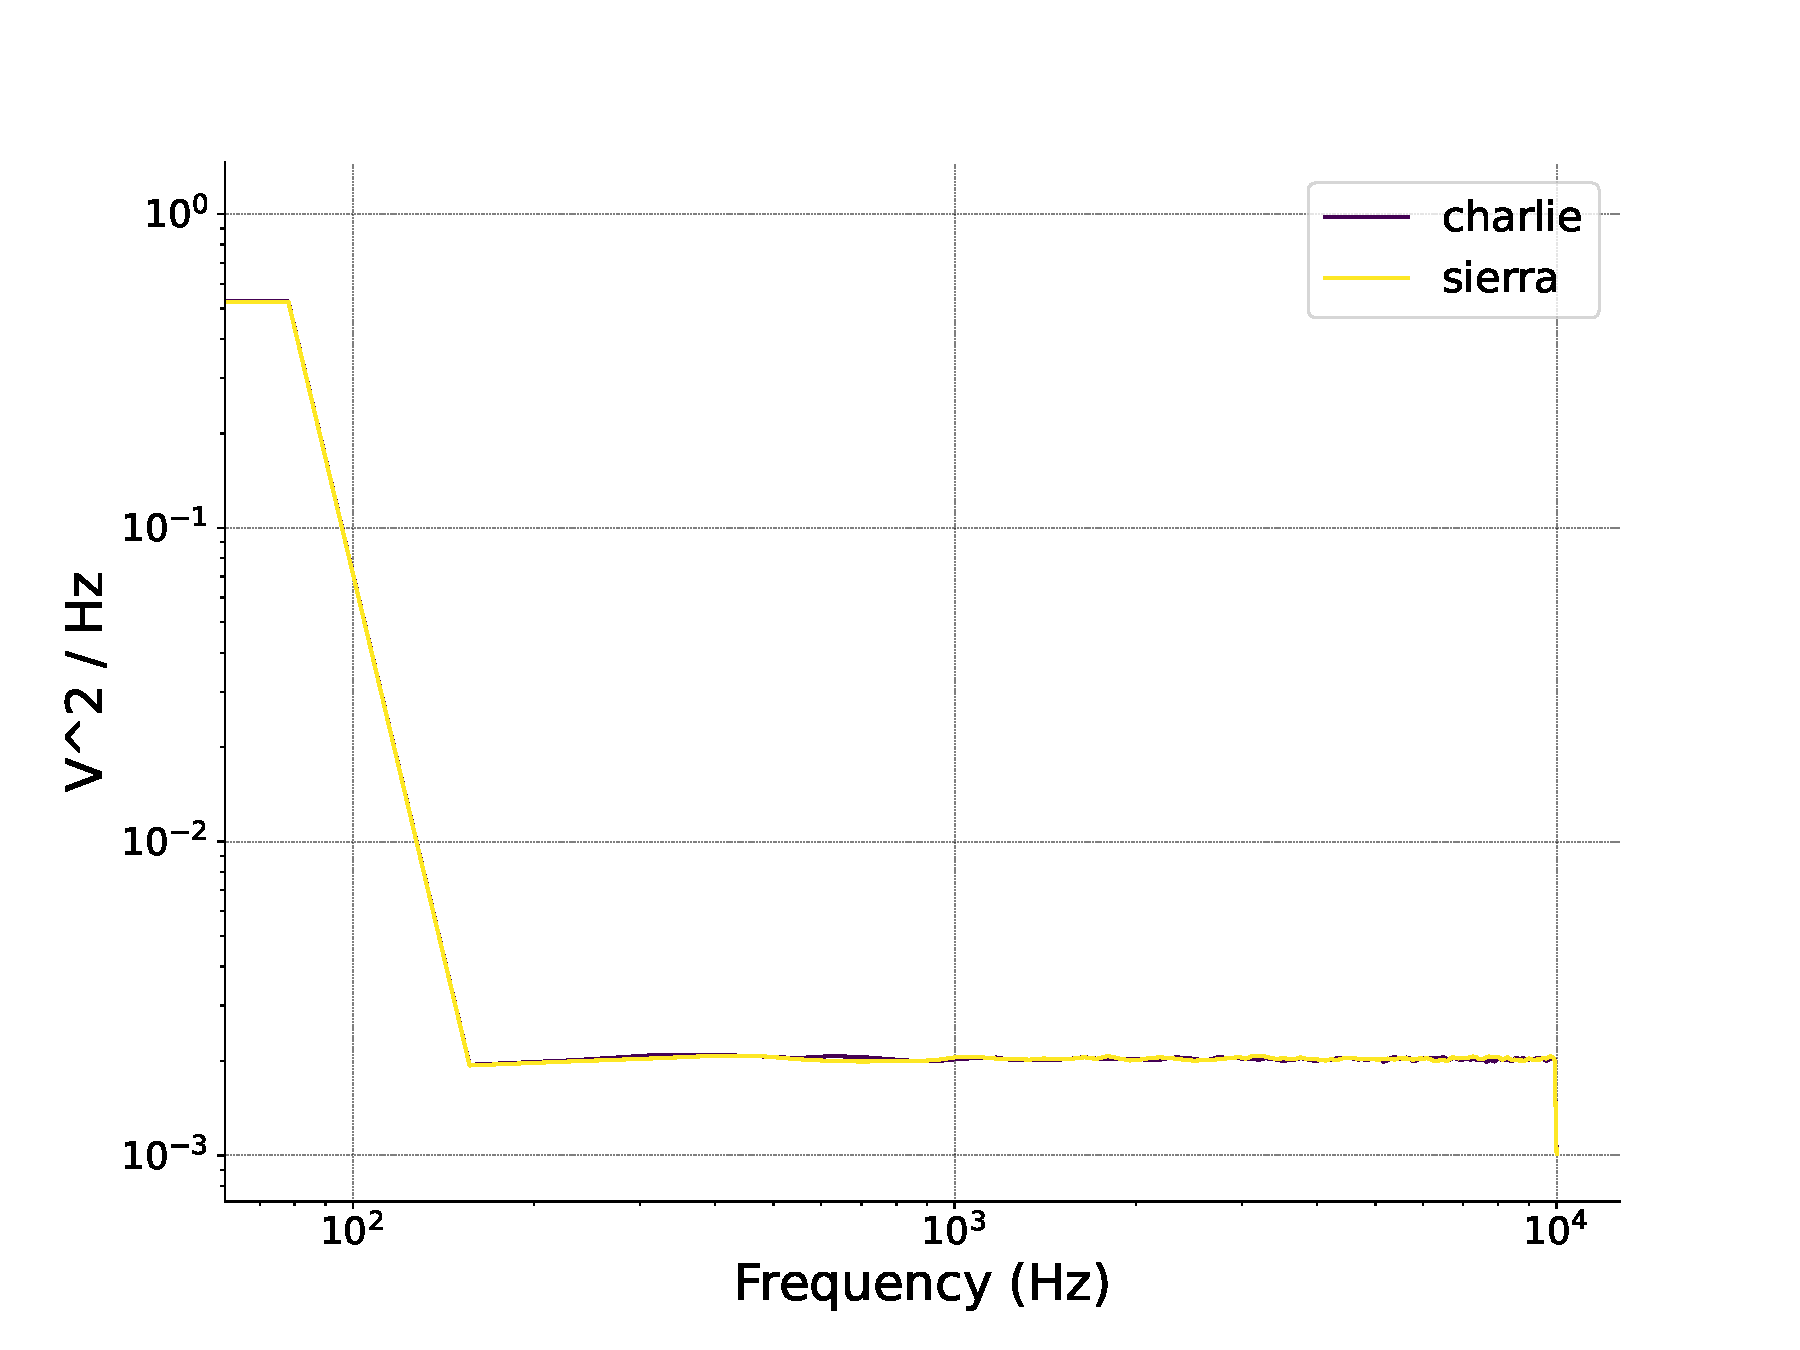
\includegraphics[width=\linewidth]{nu_ext_76PSD_homeostasis.pdf}
    \caption{Power spectral density}
    \label{charlie76PSD}
\end{figure}

Another set of comparisons is presented in Figures \ref{charlie72ratevstime} and \ref{charlie72alphavstime}, where the difference between the 2D structured one and the random one is more distinct. There the external excitation rate is set as $\nu_{ext} =  72.$
\begin{figure}[htb!] 
    \centering
    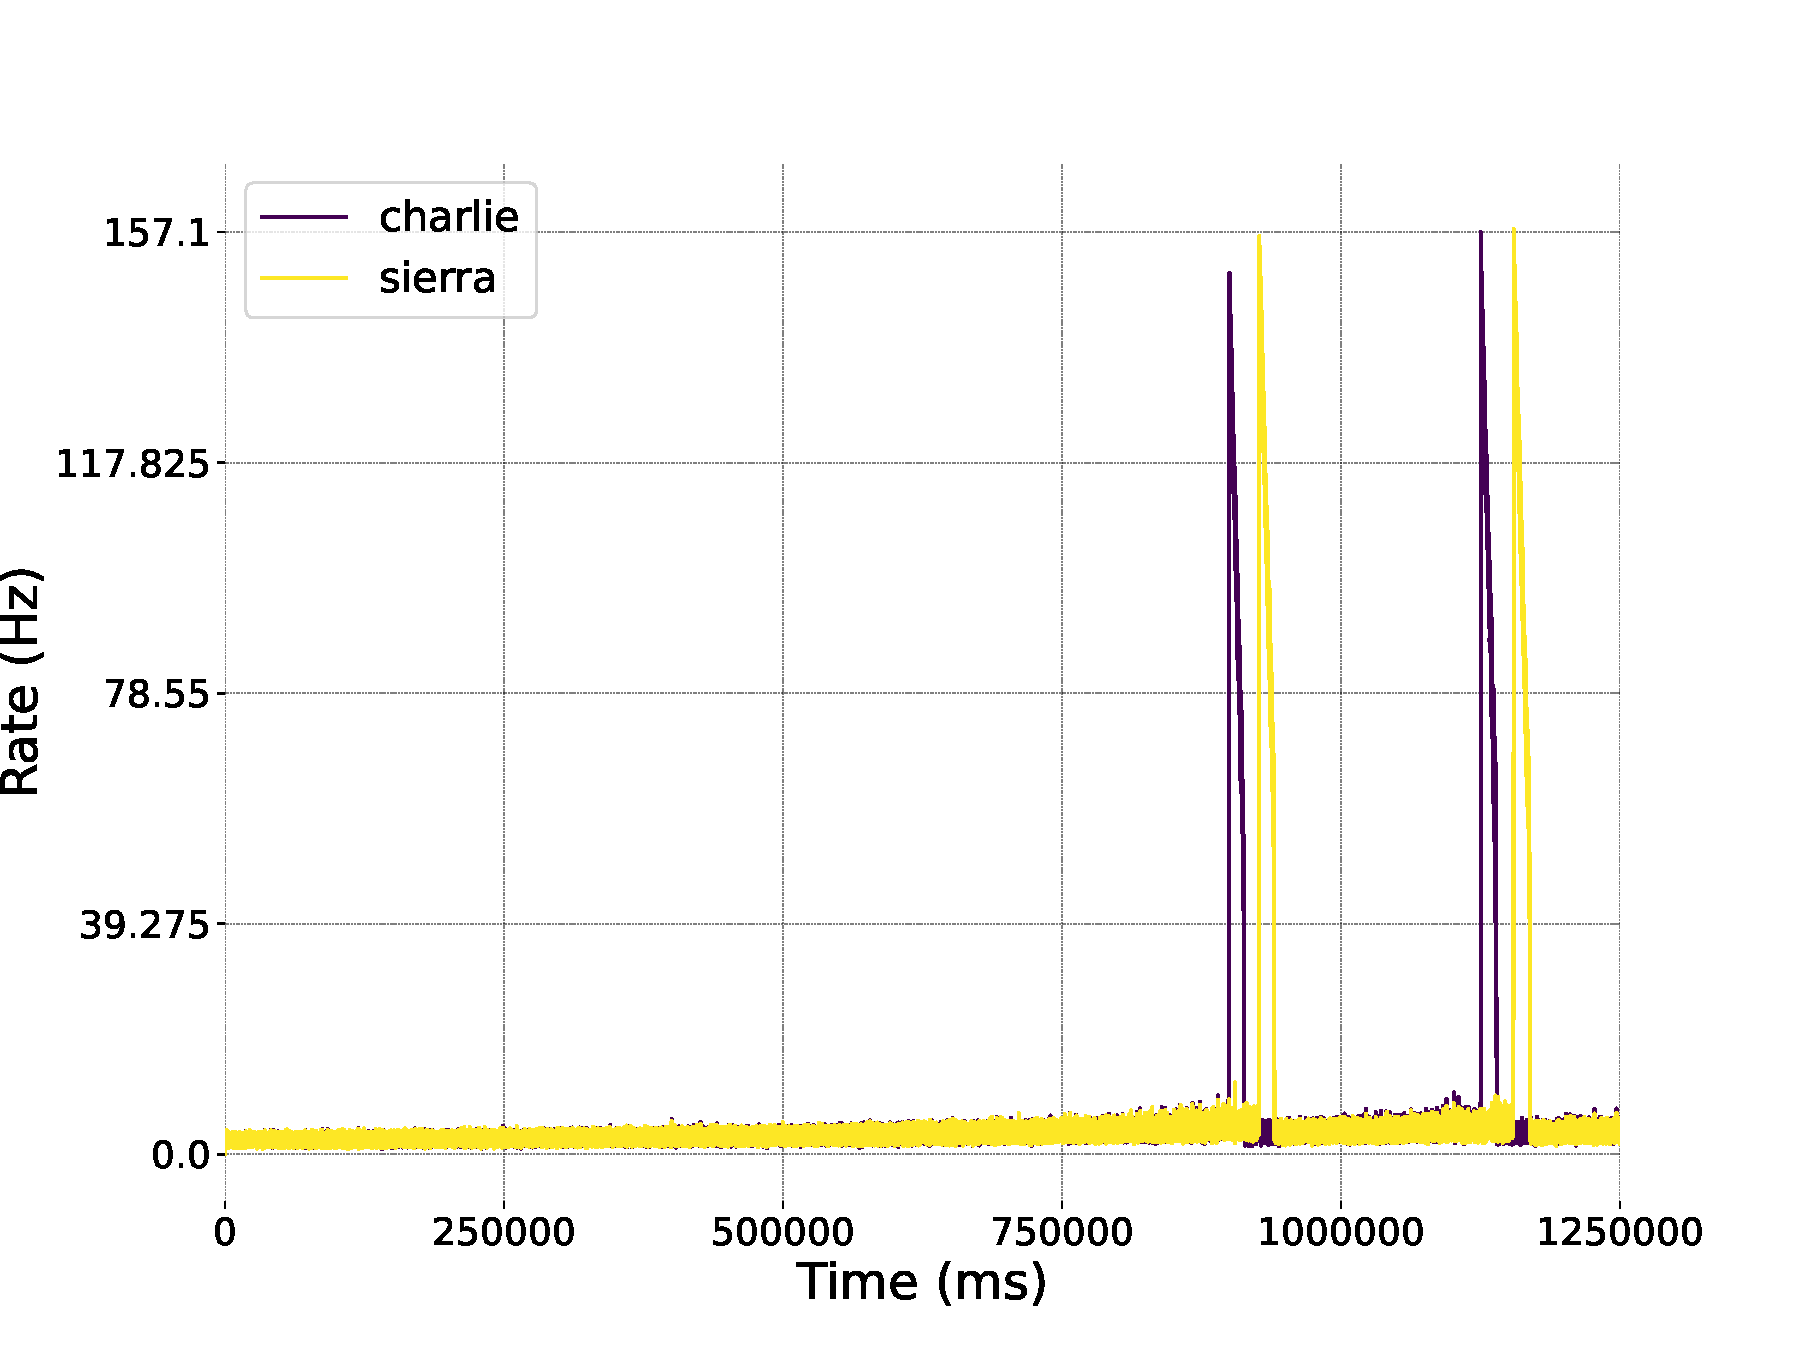
\includegraphics[width=\linewidth]{nu_ext_72rate_over_time_homeostasis.pdf}
    \caption{Rate (Hz) vs Time (ms) for $\nu_{ext} = 72$.}
    \label{charlie72ratevstime}
\end{figure}
\begin{figure}[htb!] 
    \centering
    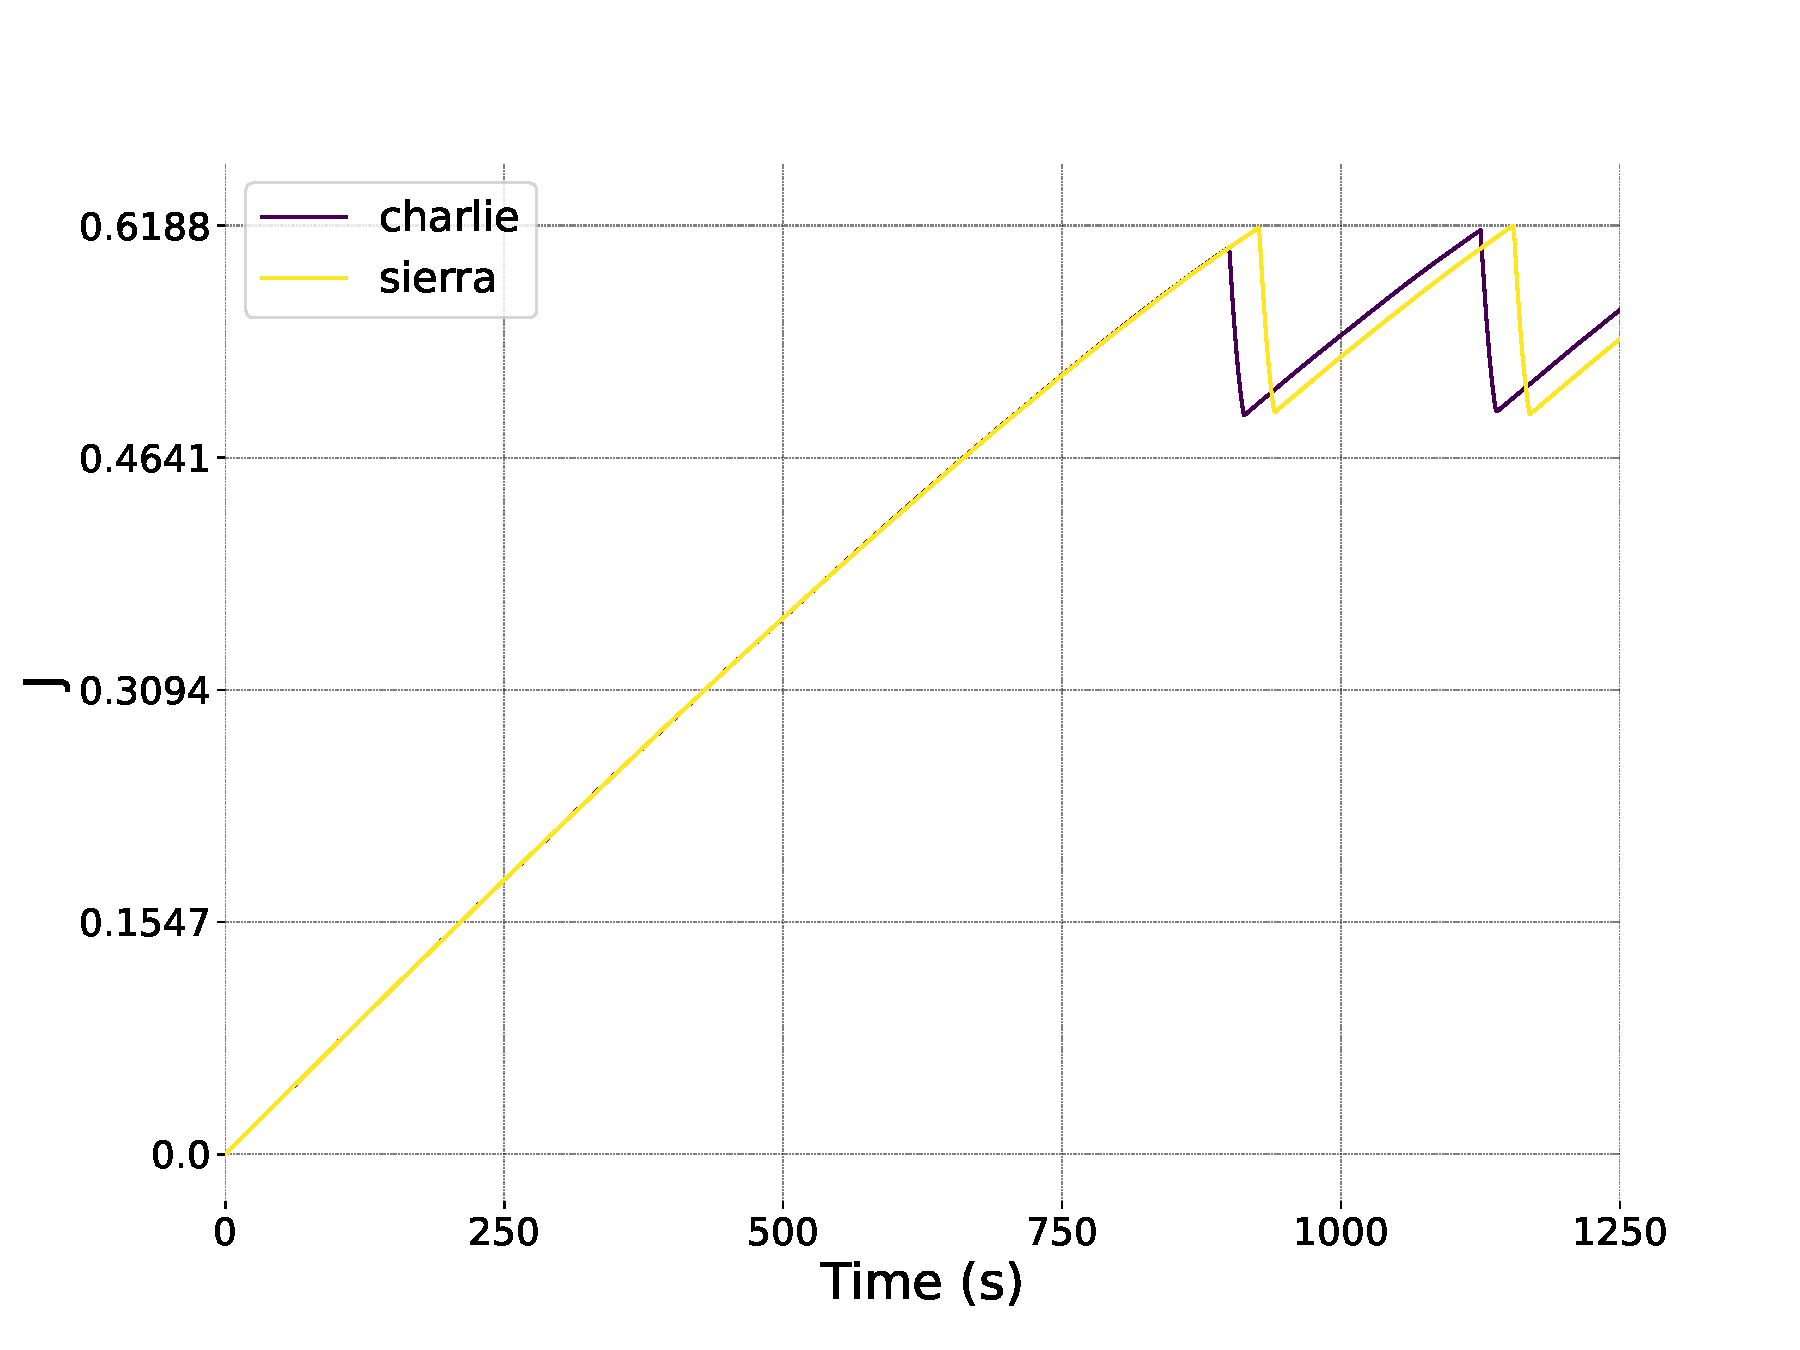
\includegraphics[width=\linewidth]{nu_ext_72alpha_over_time_homeostasis.pdf}
    \caption{J (mV) vs Time (ms) for $\nu_{ext} = 72$.}
    \label{charlie72alphavstime}
\end{figure}
It can be interpreted that the 2D structured system is more responsive than the randomly connected one. In other words, the "charlie" charged up quicker than the "Sierra".

\subsubsection{External synapse adaptation.}
The adaptation of the external synaptic coupling strengths is also implemented. The mechanism for the external regulation is identical to the inter-neuron homeostasis. In Figure, \ref{foxtrot}, the average population rate versus external Poisson input rate is presented. It can be inferred that as the external rate exceeds a specific rate of 72 in this case, the external regulation solves the problem by adjusting the couplings (weights). It can be said that for this setup, the system is purely input-driven and shows no self-regulated sustaining collective network activity.

\begin{figure}[htb!] 
    \centering
    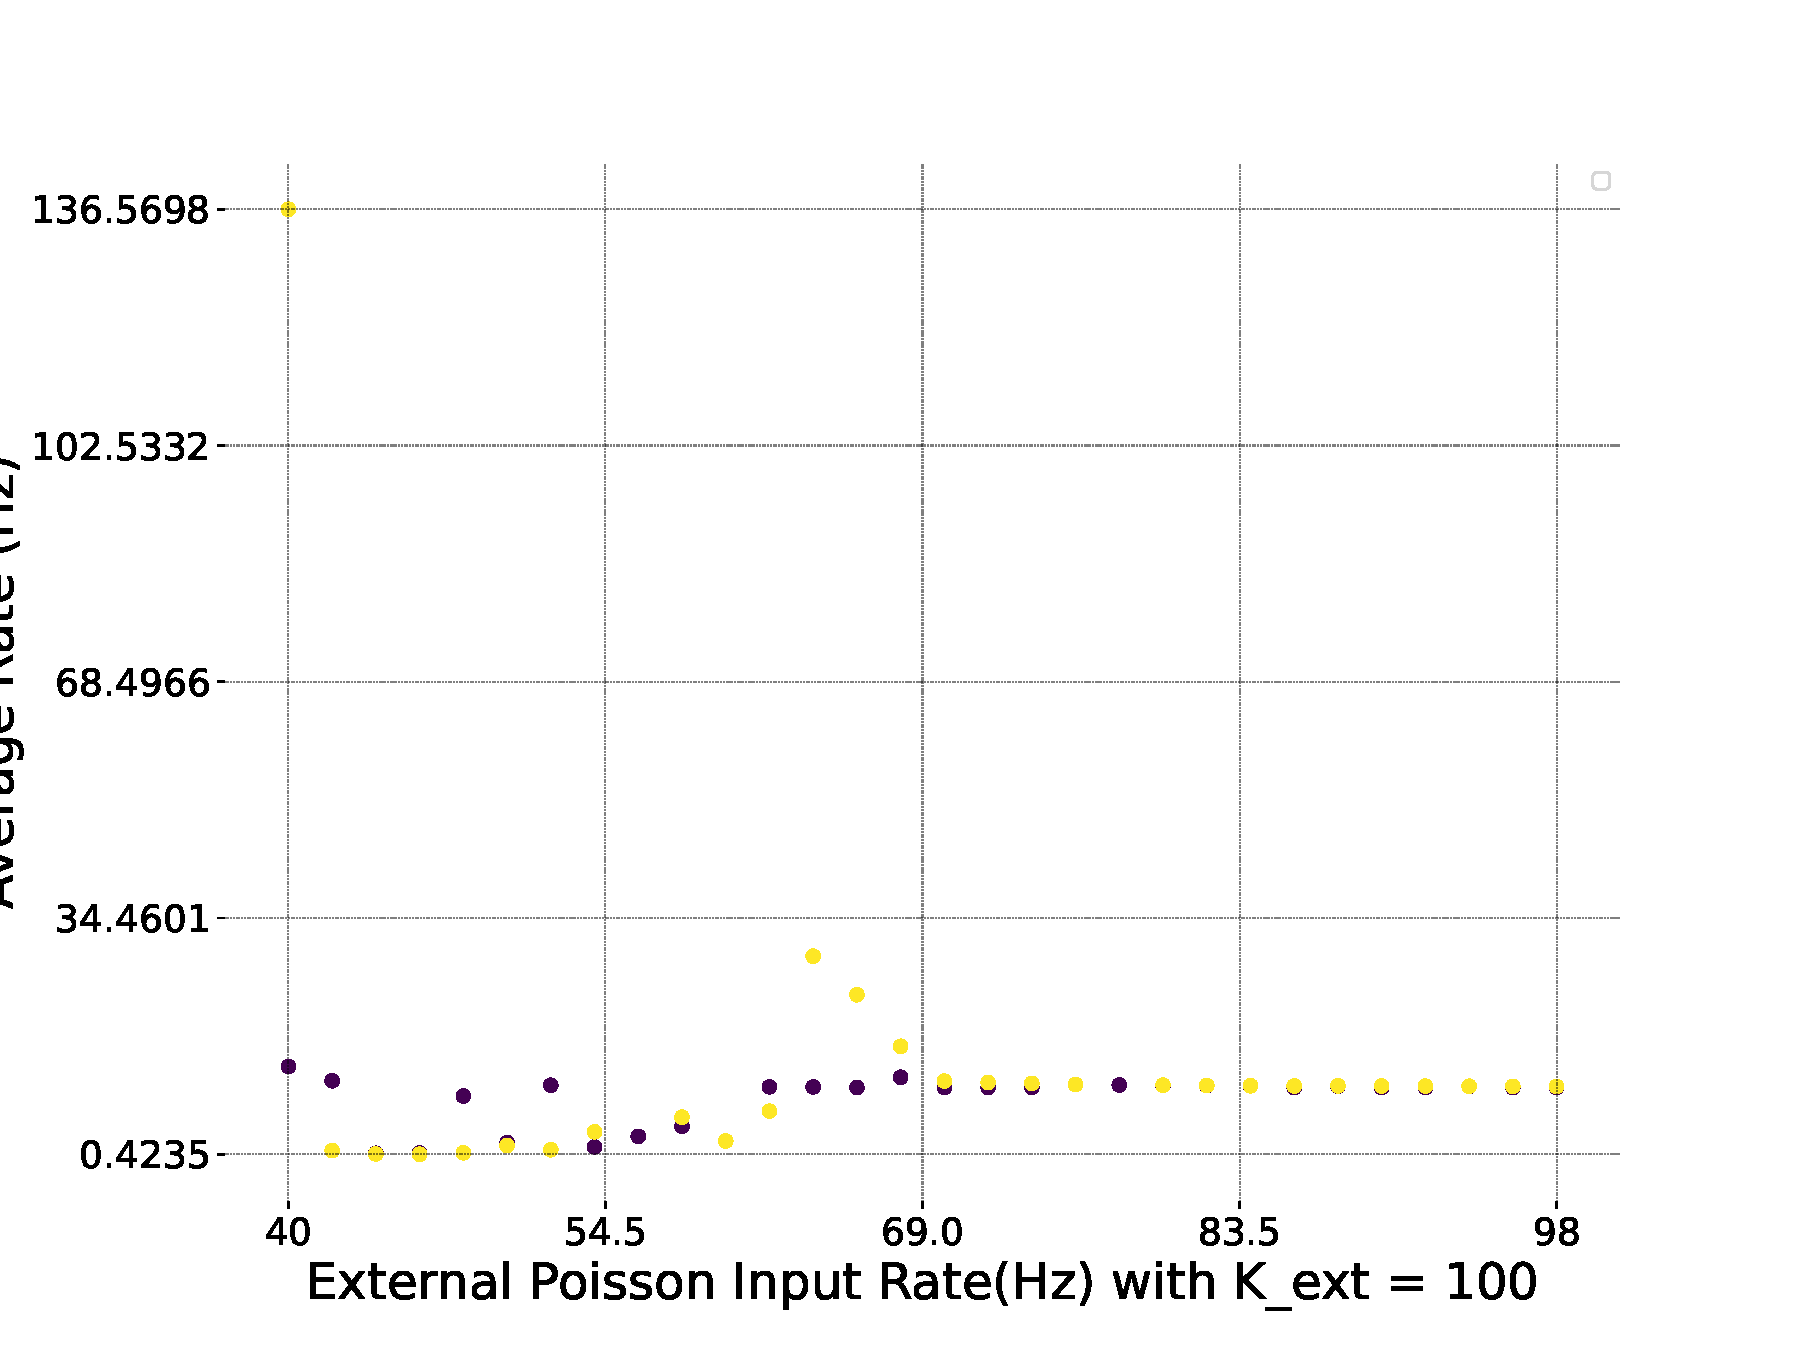
\includegraphics[width=\linewidth]{nuext_vs_activity_foxtrot.pdf}
    \caption{$\nu_{ext}$ vs Rate (Hz) for external adaptation enabled case.}
    \label{foxtrot}
\end{figure}
Figure \ref{foxtrot76PSD} presents the power spectral density for external rate $\nu_{ext} = 76$. Similarly, this PSD also carries a preliminary function.
\begin{figure}[htb!] 
    \centering
    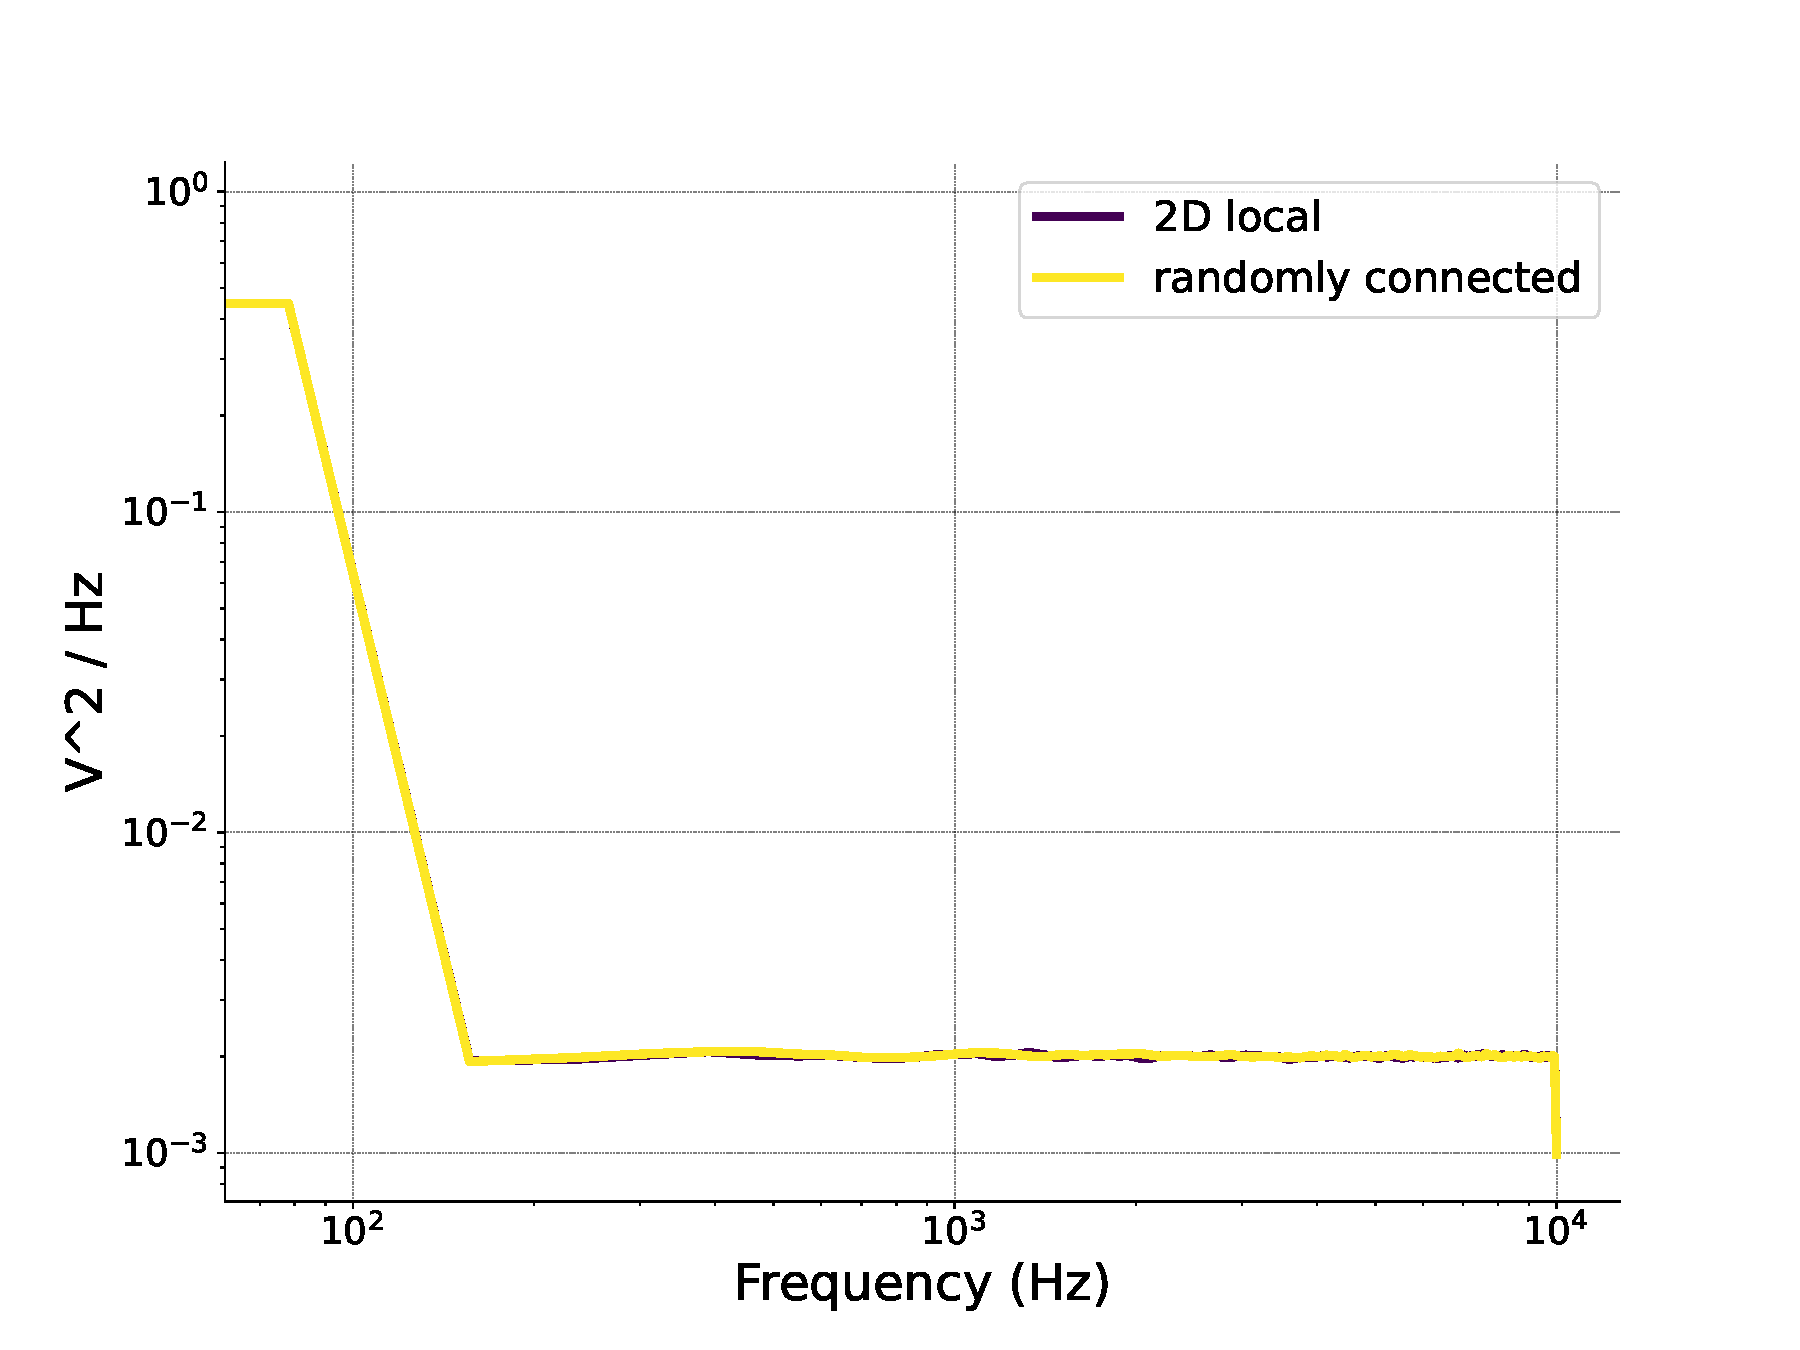
\includegraphics[width=\linewidth]{nu_ext_76PSD_homeostasis_foxtrot.pdf}
    \caption{Power spectral density for external adaptation enabled.}
    \label{foxtrot76PSD}
\end{figure}

\subsection{Future Projection on the Project}

\section{References}
\bibliography{refs/cite}

\section{Appendix}

\end{document}

%%%%%%%%%%%%%%%%%%%%%%   EXAMPLE TABLE   %%%%%%%%%%%%%%%%%%%%%%%%%%%%%%%%
\begin{table}[H]
\begin{center}
    \caption{Resistance reading by color code convention.}
    \vspace{2mm}
    \begin{tabular}{||c | c | c||} 
        \hline
        Color Order & Value & Tolerance \\ [0.5ex] 
        \hline\hline
        Brown / Black / Red / Gold & 1k\( \Omega \) & \( \% \) 5  \\ 
        \hline
        Yellow / Violet / Red / Gold & 4.7k\( \Omega \) & \( \% \) 5   \\
        \hline
        Brown / Grey / Orange / Gold & 18k\( \Omega \) & \( \% \) 5  \\ [1ex] 
        \hline
    \end{tabular}
\end{center}
\end{table}


%%%%%%%%%%%%%%%%%%%%%%   EXAMPLE IMAGE   %%%%%%%%%%%%%%%%%%%%%%%%%%%%%%%%
\begin{figure}[H]
\centering
\includegraphics[width = 1\textwidth]{5.png}
\caption{Circuit schematic for step 5}
\end{figure} 

%%%%%%%%%%%%%%%%%%%%%%   EXAMPLE IMAGE FROM PDF   %%%%%%%%%%%%%%%%%%%%%%%%%%%%%%%%
\begin{figure}[H] \centering{
    \includegraphics[scale=0.25]{2a_plot.pdf}}
    \caption{Experiment 2}
\end{figure}
